\documentclass[11pt]{amsart}

\usepackage[T1]{fontenc}
\usepackage{lmodern}
\usepackage[a4paper,hmargin=1.15in,vmargin=1.1in]{geometry}
\usepackage{amssymb,mathrsfs}
\usepackage{graphicx}
\usepackage{booktabs}
\usepackage{xcolor}
\usepackage{enumitem}
\usepackage{microtype}
\usepackage[colorlinks=true,linkcolor=blue!50!black,citecolor=blue!50!black,urlcolor=blue!50!black,bookmarks=false]{hyperref}
\usepackage{xurl}

\tolerance=2000
\emergencystretch=3em
\hfuzz=1pt
\raggedbottom

\newtheorem{theorem}{Theorem}[section]
\newtheorem{lemma}[theorem]{Lemma}
\newtheorem{proposition}[theorem]{Proposition}
\newtheorem{corollary}[theorem]{Corollary}
\newtheorem{mainthm}{Theorem}
\renewcommand{\themainthm}{\Alph{mainthm}}
\theoremstyle{definition}
\newtheorem{definition}[theorem]{Definition}
\theoremstyle{remark}
\newtheorem{remark}[theorem]{Remark}
\numberwithin{equation}{section}

\newcommand{\R}{\mathbb{R}}
\newcommand{\Z}{\mathbb{Z}}
\newcommand{\C}{\mathbb{C}}
\newcommand{\E}{\mathbb{E}}
\newcommand{\SU}{\mathrm{SU}}
\newcommand{\SO}{\mathrm{SO}}
\newcommand{\U}{\mathrm{U}}
\newcommand{\g}{\mathfrak{g}}
\newcommand{\Tr}{\operatorname{Tr}}
\newcommand{\ReTr}{\operatorname{Re}\operatorname{Tr}}
\newcommand{\Hess}{\operatorname{Hess}}
\newcommand{\Ric}{\operatorname{Ric}}
\newcommand{\Cov}{\operatorname{Cov}}
\newcommand{\Var}{\operatorname{Var}}
\newcommand{\dist}{\operatorname{dist}}
\newcommand{\ip}[2]{\langle #1,#2\rangle}
\newcommand{\BP}{\mathrm{BP}}

\begin{document}
\hypersetup{pdftitle={Yang-Mills Theory and the Mass Gap}}

\title{Yang--Mills Theory and the Mass Gap}

\author[D. Bhattacharjee]{Deep Bhattacharjee$^{*}$}
\address{Formerly, Electro-Gravitational Space Propulsion Laboratory
(EGSPL), Bhubaneswar, Odisha 751030, India; formerly, University of Calcutta (Heramba Chandra College), 23/49 Gariahat
Road, Golpark, Kolkata 700029, West Bengal, India}
\email{itsdeep@live.com, d.bhattacharjee@erl-forschung.de, egspl@proton.me}
\urladdr{\href{https://orcid.org/0000-0003-0466-750X}{orcid.org/0000-0003-0466-750X}}
\thanks{$^{*}$Corresponding author: Deep Bhattacharjee, itsdeep@live.com.}

\author[U. Bhattacharya]{Ushashi Bhattacharya}
\address{Formerly, National Taiwan University, Taipei 106319, Taiwan}
\email{rai.bhattacharya.in@gmail.com}
\urladdr{\href{https://orcid.org/0009-0002-2254-3914}{orcid.org/0009-0002-2254-3914}}

\author[J. M. Lockwood]{James Montgomery Lockwood}
\address{Independent Researcher, San Antonio, USA}
\email{spectralityworkinggroup@gmail.com}

\author[T. Romanov]{Tristan Romanov}
\address{Independent Researcher, San Francisco, CA, USA}
\email{romanov360@gmail.com}

\author[S. Singha Roy]{Sanjeevan Singha Roy}
\address{Department of Physics, Birla Institute of Technology, Mesra, Ranchi,
Jharkhand 835215, India}
\email{sanjeevan9905@gmail.com}
\urladdr{\href{https://orcid.org/0000-0002-6148-1421}{orcid.org/0000-0002-6148-1421}}

\date{10 November 2026}

\subjclass[2020]{81T25, 82B20, 81T13, 60K35, 22E30. PACS 11.15.Ha, 11.15.Tk, 05.50.+q}
\keywords{Lattice gauge theory, mass gap, Bakry--\'Emery criterion,
Dobrushin uniqueness, continuum limit}

\begin{abstract}
For four-dimensional lattice Yang--Mills theory with a compact simple gauge
group $G\subset\U(N)$ and Ricci curvature $\kappa_G$ we prove the lattice mass gap
$m\ge\operatorname{arccosh}\bigl(1+\frac1{12}\bigl(\frac{\kappa_G}{N\beta}
-\frac{29}2\bigr)\bigr)$ whenever $N\beta<\frac2{29}\kappa_G$. We prove that a
spectral gap $\varpi$ of the dynamics that resamples cubes of physical size
$\ell$, uniform in the lattice spacing, gives every nontrivial continuum limit
the mass gap $\Delta\ge16\varpi/(625e^2\ell)$, and that this cube gap holds at
strong coupling and for massive free fields; along the weak-coupling tuning
that the continuum problem requires it remains open.
\end{abstract}

\maketitle

\section{Introduction}\label{sec:intro}

The Yang--Mills existence and mass gap problem asks for a quantum
Yang--Mills theory on $\R^4$ with a compact simple gauge group that satisfies
the axioms of constructive quantum field theory, and for a number $\Delta>0$
such that the spectrum of the Hamiltonian lies in $\{0\}\cup[\Delta,\infty)$
\cite{JW06}. In the Euclidean formulation the theory is a probability measure
on gauge fields whose Schwinger functions satisfy the Osterwalder--Schrader
axioms \cite{OS73,OS75}; the mass gap is then exponential decay of the
truncated two-point functions of gauge-invariant observables at the rate
$\Delta$. The natural regularisation is Wilson's lattice gauge theory
\cite{Wil74}: an element $Q_e$ of $G\subset\U(N)$ sits on every link $e$ of the
lattice $a\Z^4$, and a configuration has the weight
$\exp(N\beta\sum_p\ReTr Q_p)$, where $Q_p$ is the ordered product around the
plaquette~$p$.\footnote{This is the normalisation of~\cite{SZZ23,BB26a}. The
conventional inverse coupling is $\beta_W=N^2\beta$, and for $\SU(2)$,
identified with the unit quaternions, $\beta_W=4\beta$.} Asymptotic freedom
forces the continuum limit $a\to0$ to be taken with $\beta\to\infty$, that is,
at weak coupling.

At small $\beta$ the lattice theory has a unique state, exponential clustering
and a transfer-matrix gap, by convergent expansions \cite{OSei78,Sei82};
Ba{\l}aban's renormalisation group \cite{Bal84a,Bal85a,Bal89b}, as presented by
Dimock \cite{Dim13}, gives ultraviolet stability in finite volume at weak
coupling, and Magnen, Rivasseau and S\'en\'eor constructed the theory with an
infrared cutoff \cite{MRS93}. No existing result gives a mass gap in physical
units. This paper proves three things about this problem, and states
precisely what is missing.

\subsection{The lattice gap with explicit constants}

Let $G$ be a compact connected Lie group with semisimple Lie algebra,
identified with its image under a faithful unitary representation in $\U(N)$,
and let $\kappa_G>0$ be its least Ricci curvature for the bi-invariant metric
$\ip XY=-\Tr(XY)$. For a simple group $\kappa_G=h^\vee/(2\ell_\rho)$, with $h^\vee$
the dual Coxeter number and $\ell_\rho$ the Dynkin index of the representation;
for $\SU(N)$, $\kappa_G=N/2$.

\begin{mainthm}\label{thm:A}
Suppose $N|\beta|<\frac2{29}\kappa_G$. For every gauge-invariant local
observable the expectations in boxes with free boundary converge, along every
exhausting sequence of boxes, to a state $\omega$ that is invariant under the
lattice symmetries; truncated correlations of Lipschitz observables decay at
every rate below
\[
m_G(\beta)=\operatorname{arccosh}\Bigl(1+\frac1{12}\Bigl(\frac{\kappa_G}{N|\beta|}
-\frac{29}2\Bigr)\Bigr)>0 ,
\]
and for $\beta\ge0$ the state is reflection positive and its transfer matrix
has spectral gap $m\ge m_G(\beta)$. For $G=\SU(2)$ the same holds for
$|\beta_W|<\frac13$ with $m\ge-\log(3\beta_W)$.
\end{mainthm}

Two ingredients carry the proof. The first is a gauge: a field of straight
lines on $\Z^4$ that contains exactly one link of every plaquette
(Sec.~\ref{sec:linefield}). Setting these links to the identity loses no
gauge-invariant information, and every remaining link then interacts with
exactly twelve others instead of eighteen. The second is a Hessian bound in
this gauge, $|\Hess S|\le\frac{29}2$ for the action $S=\sum_p\ReTr Q_p$, proved
by a divergence identity and a positivity statement for one plaquette
(Sec.~\ref{sec:curvature}); with the Ricci curvature of $G$ it gives a
Bakry--\'Emery bound \cite{BE85,BGL14} with an explicit decay rate. Without
the gauge the sharp Hessian bound is $16$ \cite{BB26a}, so the gauge enlarges
the range of every group by the factor $32/29$ and supplies the rate. The
$\SU(2)$ statement combines the gauge with the sharp Kantorovich modulus
$\frac14$ of the von Mises--Fisher family \cite{BB26a} in Dobrushin's
criterion \cite{Dob68,Dob70}.

\subsection{A continuum mass gap from one cube}

The lattice gap of Theorem~\ref{thm:A} is measured in lattice units and
vanishes in physical units as $a\to0$. The second result isolates a single
estimate, posed on one scale, that controls the gap in physical units. On a
periodic lattice let $\mathcal P_x$ resample the links of the cube of side $n$
at $x$ from their conditional law under the Wilson measure $\mu$. The
condition $\BP(n,\varpi)$ asks that
\[
\varpi\Var_\mu(f)\le\frac1{n^4}\sum_x\mu\bigl((f-\mathcal P_xf)^2\bigr)
\]
for every gauge-invariant $f$: the dynamics that resamples cubes, each link
at rate one, has spectral gap at least $\varpi$ on gauge-invariant functions.
The condition involves no gauge fixing and no supremum over boundary
conditions.

\begin{mainthm}\label{thm:B}
Let $a_k\to0$ and $\beta_k\ge0$ be couplings, and suppose that there are
$\varpi>0$, $\ell>0$ and integers $n_k\ge2$ with $n_ka_k\le\ell$ such that
$\BP(n_k,\varpi)$ holds for the Wilson measure at $\beta_k$ on all large tori.
Then every continuum limit of the corresponding lattice theories has
Hamiltonian $H$ with $\sigma(H)\subset\{0\}\cup[\Delta,\infty)$,
\[
\Delta=\frac{16\varpi}{625e^2\ell},
\]
and $0$ is a simple eigenvalue; if the limit is nontrivial, $H$ has a mass
gap of at least $\Delta$.
\end{mainthm}

The proof (Sec.~\ref{sec:cube}) turns the spectral gap into decay of
covariances through a finite-speed bound for the cube dynamics, at a rate
of order $1/n$ in lattice units, hence of order $1/\ell$ in physical units,
and passes this decay through the Osterwalder--Schrader reconstruction.

\subsection{Where the cube condition holds}

\begin{mainthm}\label{thm:C}
\begin{enumerate}[label=\textup{(\roman*)},leftmargin=*]
\item At $\beta=0$, $\BP(n,1)$ holds for every $n$. For
$21N|\beta|<\kappa_G$ and $n$ large, $\BP(n,1-\alpha_n)$ holds with
$\alpha_n=N|\beta|(18n-3)/((\kappa_G-21N|\beta|)n^2)\to0$; for $\SU(2)$ the
range is $|\beta_W|<\frac4{15}$.
\item For the free scalar field of lattice mass $\mu$ in $d$ dimensions the
best constant is
$\varpi=\frac{\mu^2}{n^d}\ip{\mathbf 1}{(-\Delta_D+\mu^2)^{-1}\mathbf 1}$, with
$-\Delta_D$ the Dirichlet Laplacian of the cube, and with $s=n\mu$ (the mass
times the physical size of the cube)
\[
\Bigl(\frac56\Bigr)^d\frac{s^2}{s^2+10d}\le\varpi\le\frac{s^2}{s^2+16d/9}.
\]
\end{enumerate}
\end{mainthm}

Part (ii) is the model case of the continuum tuning: the constant is uniform
in the lattice spacing at fixed $m\ell$, and it vanishes as $m\to0$. The cube
condition is therefore a quantitative statement of mass generation at the
scale $\ell$.

\subsection{What remains}

Theorem~\ref{thm:A} is a strong-coupling theorem. The Clay problem needs the
opposite end of the coupling range: the continuum limit lives at
$\beta\to\infty$, where the range $N\beta<\frac2{29}\kappa_G$ of
Theorem~\ref{thm:A} and the range of Theorem~\ref{thm:C}(i) do not reach. Two
statements would complete the proof of a continuum mass gap, and neither is
proved here:
\begin{enumerate}[label=\textup{(\Alph*)},leftmargin=*]
\setcounter{enumi}{3}
\item $\BP(n_k,\varpi)$ with $n_ka_k\le\ell$ along the asymptotic-freedom
tuning $\beta_k\to\infty$, uniformly in $k$;
\item convergence of the renormalised Schwinger functions to a nontrivial
limit satisfying the Osterwalder--Schrader axioms.
\end{enumerate}
Given (D) and (E), Theorem~\ref{thm:B} gives the mass gap $\Delta\ge
16\varpi/(625e^2\ell)$. Section~\ref{sec:weak} explains why (D) is the heart of
the matter: by Theorem~\ref{thm:C}(ii) it cannot hold without a dynamically
generated mass, it fails at fixed cube size at weak coupling, and it fails in
the Coulomb phase of the abelian theory, so its proof has to use the
non-abelian structure of $G$ at every scale up to $\ell$.

\subsection{Related work}

Strong-coupling clustering goes back to Osterwalder and Seiler \cite{OSei78}
and Seiler \cite{Sei82}; probabilistic treatments include the survey of
Chatterjee \cite{Chat19}, the Langevin approach of Shen, Zhu and Zhu
\cite{SZZ23}, whose Bakry--\'Emery argument we sharpen, the area law in
enlarged regions of Cao, Nissim and Sheffield \cite{CNS25}, and correlation
decay for finite gauge groups at weak coupling by Adhikari and Cao \cite{AC25}.
In two dimensions the continuum measure is known
\cite{GKS89,Dri89,Lev03}. The Kantorovich modulus of the $\SU(2)$ single-link
law and the sharp Hessian bound without gauge fixing are proved in
\cite{BB26a}, and an earlier and much longer account of the one-cube
reduction is \cite{BBLR26}.

I.~J.~Sessford~\cite{Ses26} has formalised in Lean~4 with Mathlib, without
unproved statements and with only the standard axioms, several ingredients of
the strong-coupling analysis on periodic lattices: the Haar probability on
$\SU(N)$, an infinite-volume Gibbs state obtained as a limit of torus states,
site reflection positivity and the transfer matrix, the Holley--Stroock
comparison, Dobrushin's covariance bounds, and the passage from decay of
correlations to a transfer-matrix gap (one direction of
Proposition~\ref{prop:gapdecay}). For the periodic state it proves a
transfer-matrix gap for every $N$ at $\beta_W<5.9\cdot10^{-5}$, and explicit
single-link heat-bath gaps on boxes of side fifteen for $\SU(2)$ at
$\beta_W\le0.166$ and for $\SU(3)$ at $\beta_W\le0.38$ (his coupling is
$\beta_W/2$). It also proves, by a Poincar\'e inequality and a light-cone
argument different from Lemma~\ref{lem:speed}, that an ungauged one-cube
influence condition gives a lattice gap of order $1/n$; this is a variant of
the lattice step, Theorem~\ref{thm:decay} and Corollary~\ref{cor:latticegap},
at a smaller rate. The continuum step, the gauge
fixing and the curvature bounds are not part of that development, which shares
with this paper the open hypothesis (D).

\section{Lattice gauge theory and the transfer matrix}\label{sec:lattice}

Write $e_0,\dots,e_3$ for the unit vectors of $\Z^4$, $(x,\mu)$ for the link
from $x$ to $x+e_\mu$, and $Q_{(x,\mu)}^{-1}$ for the variable of the reversed
link. A box $\Lambda$ is a product of four finite intervals, with its set
$E(\Lambda)$ of links and its set $P(\Lambda)$ of plaquettes. For a plaquette
at $x$ in the plane $\mu<\nu$ with links $e_1=(x,\mu)$, $e_2=(x+e_\mu,\nu)$,
$e_3=(x+e_\nu,\mu)$, $e_4=(x,\nu)$, put $Q_p=Q_{e_1}Q_{e_2}Q_{e_3}^*Q_{e_4}^*$.
With $dQ$ the Haar probability measure of $G$, the Wilson measure of a box
with free boundary is
\[
W_\Lambda(dQ)=\frac1{Z_\Lambda}\exp\Bigl(N\beta\sum_{p\in P(\Lambda)}\ReTr
Q_p\Bigr)\prod_{e\in E(\Lambda)}dQ_e ,
\]
and the Wilson measure $\mu_L$ of the torus $\Lambda_L=(\Z/L\Z)^4$ is defined
in the same way with all links and plaquettes of $\Lambda_L$. Both are
invariant under the gauge transformations $Q_{(x,y)}\mapsto g_xQ_{(x,y)}
g_y^{-1}$. A function of finitely many links is a local observable, and it
is gauge invariant if it is invariant under these transformations. For
$\beta\ge0$ the measures are reflection positive for reflections in lattice
hyperplanes through sites and in hyperplanes bisecting links, on boxes
symmetric under the reflection and on tori of even side~\cite{OSei78}.

Let $\omega$ be a state on the gauge-invariant local observables of $\Z^4$
that is invariant under translations and reflection positive in this sense.
The Osterwalder--Schrader construction~\cite{OS73,OS75,OSei78} gives a
Hilbert space $\mathcal H$ with a unit vector $\Omega$, a map $F\mapsto\Psi_F$
from the observables at nonnegative times to $\mathcal H$ with dense range,
and a self-adjoint transfer matrix $0\le\mathbb T\le1$ with $\mathbb T\Omega=
\Omega$ and
\[
\ip{\Psi_F}{\mathbb T^t\Psi_H}=\omega\bigl(\vartheta(\bar F)\,\tau_tH\bigr),
\qquad t\in\Z_{\ge0},
\]
where $\vartheta$ is the time reflection and $\tau_t$ the time translation;
$\Psi_F$ is the class of $F$ for the positive semidefinite form
$\omega(\vartheta(\bar F)H)$, and $\|\Psi_F\|^2\le\omega(|F|^2)$. The
\emph{spectral gap} of $\mathbb T$ is $m$ if its spectrum on $\Omega^\perp$
lies in $[0,e^{-m}]$.

\begin{proposition}\label{prop:gapdecay}
Let $m>0$ and let $\mathcal F$ be a class of gauge-invariant local
observables, supported at nonnegative times, that is dense in $L^2(\omega)$
on each bounded time support. If for every $F\in\mathcal F$ there is
$C_F<\infty$ with
\[
\omega(\vartheta(\bar F)\tau_tF)-|\omega(F)|^2\le C_Fe^{-mt}\qquad(t\ge0),
\]
then $\mathbb T$ has spectral gap at least $m$.
\end{proposition}

\begin{proof}
Put $\Psi'_F=\Psi_F-\ip\Omega{\Psi_F}\Omega$, so that the left side equals
$\ip{\Psi'_F}{\mathbb T^t\Psi'_F}=\int\lambda^t\,d\sigma_F(\lambda)$, with
$\sigma_F$ the spectral measure of $\mathbb T$ at $\Psi'_F$. For $\delta>0$
this is at least $\sigma_F((e^{-m+\delta},1])e^{(-m+\delta)t}$, which exceeds
$C_Fe^{-mt}$ for large $t$ unless $\sigma_F((e^{-m+\delta},1])=0$. So the
spectral projection of $(e^{-m},1]$ annihilates every $\Psi'_F$. These vectors
are dense in $\Omega^\perp$, because $\|\Psi_F\|^2\le\omega(|F|^2)$ and the
class is dense, so the projection vanishes on $\Omega^\perp$.
\end{proof}

The decay of a single two-point function does not suffice: it places only
one spectral measure in $[0,e^{-m}]$, and the density of the class is what
gives the gap.

\section{The line field}\label{sec:linefield}

A \emph{direction field} is a map $\sigma:\Z^4\to\{0,1,2,3\}$; its links
are $F=\{(x,\sigma(x)):x\in\Z^4\}$. At each site put $\pi_x(\mu)=
\sigma(x+e_\mu)$. The plaquette at $x$ in the plane $\{\mu,\nu\}$ contains
\begin{equation}\label{eq:count}
[\sigma(x)\in\{\mu,\nu\}]+[\pi_x(\mu)=\nu]+[\pi_x(\nu)=\mu]
\end{equation}
links of $F$.

\begin{lemma}\label{lem:cycle}
Every plaquette contains exactly one link of $F$ if and only if, at every
site $x$, $\pi_x$ fixes $\sigma(x)$ and permutes the other three directions
cyclically.
\end{lemma}

\begin{proof}
Fix $x$, let $s=\sigma(x)$ and let $R$ be the other three directions. For the
plane $\{s,\nu\}$ the count~\eqref{eq:count} is $1+[\pi_x(s)=\nu]+[\pi_x(\nu)
=s]$, which equals one for all $\nu\in R$ exactly when $\pi_x$ fixes $s$ and
maps $R$ into $R$. For a plane $\{\mu,\nu\}\subset R$ the count is
$[\pi_x(\mu)=\nu]+[\pi_x(\nu)=\mu]$. Draw an arrow $\mu\to\pi_x(\mu)$ whenever
$\pi_x(\mu)\in R\setminus\{\mu\}$; each vertex has at most one outgoing arrow,
and the condition asks for exactly one arrow on each of the three pairs. Three
arrows on three vertices with out-degree at most one give out-degree one
everywhere, and such a tournament is a directed three-cycle.
\end{proof}

From now on $\sigma$ is the field of period two of Table~\ref{tab:sigma} in
Appendix~\ref{app:table}; in each row $\pi_x$ fixes $\sigma(x)$ and is a
three-cycle on the other directions, so every plaquette contains exactly one
link of $F$.\footnote{A field with one link of $F$ at every site and one in
every plaquette can exist only in four dimensions: a site carries
$d(d-1)/2$ plaquettes at which it is the base point and a link lies in
$2(d-1)$ plaquettes, and the two counts agree only for $d=4$.} Call the links
outside $F$ \emph{active} and write $A$ for their set.

\begin{lemma}\label{lem:structure}\leavevmode
\begin{enumerate}[label=\textup{(\roman*)},leftmargin=*]
\item $F$ is a disjoint union of bi-infinite straight lines, one through every
site; hence $F\cap E(\Lambda)$ is a forest for every box $\Lambda$.
\item An active link $e=(x,\mu)$ lies in six plaquettes. In four of them the
link of $F$ shares an end point with $e$; in the other two it is opposite to
$e$.
\item Every active link shares a plaquette with exactly twelve other active
links, two in each of its plaquettes, and two links share at most one
plaquette.
\end{enumerate}
\end{lemma}

\begin{proof}
(i) Since $\pi_x$ fixes $\sigma(x)$, $\sigma(x+e_{\sigma(x)})=\sigma(x)$, and since
$\sigma$ has period two, also $\sigma(x-e_{\sigma(x)})=\sigma(x)$. If $(x-e_\nu,\nu)
\in F$, straightness at $x-e_\nu$ gives $\sigma(x)=\nu$, so the incoming link of
$F$ at $x$ is unique and continues the outgoing one. A line meets a box in a
segment.

(ii) A link of $F$ sharing an end point with $e$ is the outgoing or incoming
link of $F$ at $x$, of direction $s=\sigma(x)\ne\mu$, or at $x+e_\mu$, of
direction $t=\pi_x(\mu)\in R\setminus\{\mu\}$. They lie in the two plaquettes of
$e$ in the plane $\{\mu,s\}$ and the two in the plane $\{\mu,t\}$, four distinct
plaquettes as $s\ne t$. In the two plaquettes of the remaining plane
$\{\mu,\rho\}$ the unique link of $F$ touches neither end of $e$, so it is the
opposite link.

(iii) Each plaquette of $e$ contains $e$, one link of $F$ and two other links.
\end{proof}

\begin{figure}[t]
\centering
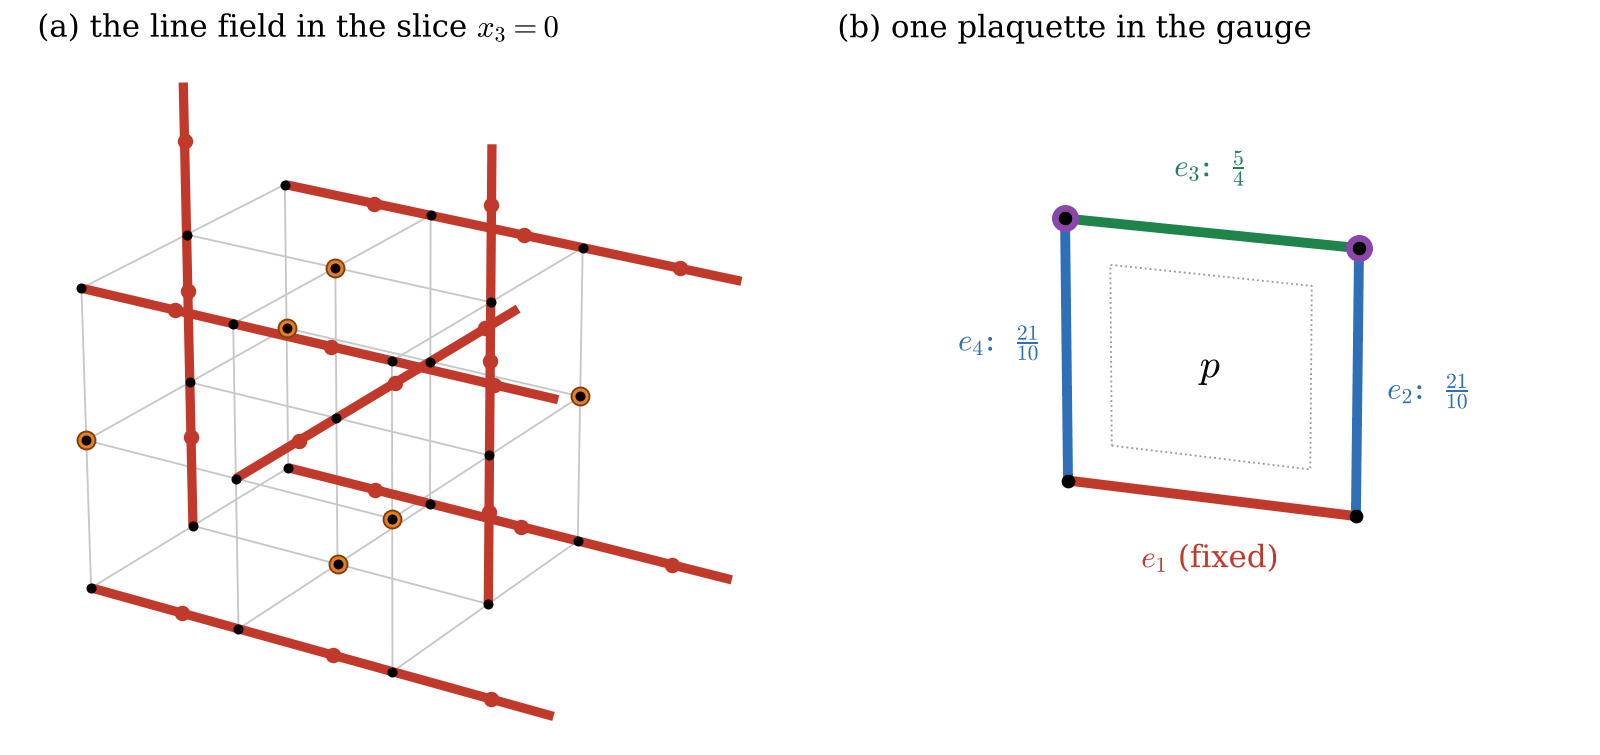
\includegraphics[width=0.92\textwidth]{fig_linefield.png}
\caption{(a) The line field in the slice $x_3=0$ of a box of side three;
thick segments are links of $F$, rings mark sites whose line leaves the slice
in direction $3$. (b) One plaquette with its fixed link $e_1$ and the weights
$\frac{21}{10}$, $\frac54$ of Lemma~\ref{lem:local} on its active links.}
\label{fig:linefield}
\end{figure}

\section{Gauge fixing and the free-boundary state}\label{sec:state}

For a function $O$ of the links let $O^F$ be $O$ with every link of $F$ set to
the identity.

\begin{lemma}[gauge fixing]\label{lem:gaugefix}
Let $\mu^F_\Lambda$ be the probability measure on $G^{A\cap E(\Lambda)}$ with
density proportional to $\exp(N\beta\sum_{p\in P(\Lambda)}\ReTr Q^F_p)$. For
every gauge-invariant $O$ on $G^{E(\Lambda)}$, $W_\Lambda(O)=\mu^F_\Lambda(O^F)$.
\end{lemma}

\begin{proof}
Each segment of $F\cap E(\Lambda)$ is a path $x_0,\dots,x_k$. Given the
variables on $F$, put $g_{x_0}=1$ and $g_{x_{i+1}}=g_{x_i}Q_{(x_i,x_{i+1})}$
along every segment. The transformed field equals the identity on $F\cap
E(\Lambda)$, and for fixed values on $F$ the map from the active variables to
the transformed ones is a product of translations, which preserve Haar
measure. Gauge invariance of the action and of $O$ gives the claim.
\end{proof}

No holonomy remains because $F\cap E(\Lambda)$ is a forest. The measures
$\mu^F_\Lambda$ are finite-volume versions of the specification $\gamma^F$ on
$G^A$ in which $\gamma^F_e$ resamples an active $Q_e$ from the law with density
proportional to $\exp(N\beta\sum_{p\ni e}\ReTr Q^F_p)$ given the other active
links. Fix a bi-invariant metric $\delta$ on $G$ of diameter $D$ and define the
Kantorovich coefficients
\[
C_{ee'}=\sup\frac{W_1\bigl(\gamma^F_e(\cdot\mid Q),\gamma^F_e(\cdot\mid Q')\bigr)}
{\delta(Q_{e'},Q'_{e'})},
\]
the supremum over configurations that differ only at $e'$; $W_1$ is the
Kantorovich distance~\cite{Vil09}, and $C_{ee'}=0$ unless $e$ and $e'$ share a
plaquette.

\begin{lemma}[comparison]\label{lem:comparison}
Suppose every row and column of $(C_{ee'})$ sums to at most $\alpha<1$, and let
$\lambda>0$ with $\theta=\alpha e^\lambda<1$. Let $S\subset A$ and let $\mu_1,\mu_2$
be probability measures on $G^A$ invariant under $\gamma^F_e$ for $e\notin S$.
Let $T\subset A\setminus S$ be finite, $w_b=e^{-\lambda\dist(b,T)}$ with the
distance of link midpoints, and suppose $\sum_{z\in S}w_z<\infty$. There is a
coupling of $\mu_1$ and $\mu_2$ with $\varrho(b)=\E\,\delta(\sigma_b,\sigma'_b)$
satisfying
\[
\sum_{b\notin S}w_b\varrho(b)\le\frac{\theta D}{1-\theta}\sum_{z\in S}w_z ,
\]
and $\mu_1=\mu_2$ if $S=\emptyset$.
\end{lemma}

\begin{proof}
The couplings form a weakly compact set on which $\Psi(\pi)=\sum_bw_b\E_\pi
\delta(\sigma_b,\sigma'_b)$ is continuous; let $\pi^*$ minimise it. For $e\notin S$
replace $(\sigma_e,\sigma'_e)$ by a sample of an optimal coupling of
$\gamma^F_e(\cdot\mid\sigma)$ and $\gamma^F_e(\cdot\mid\sigma')$, chosen
measurably~\cite[Cor.~5.22]{Vil09}. Both $\mu_i$ are invariant, so this is again
a coupling, and changing the links that enter $\gamma^F_e$ one at a time gives
$\varrho(e)\le\sum_{e'}C_{ee'}\varrho(e')$ by minimality. Multiply by $w_e$ and sum
over $e\notin S$; where $C_{ee'}\ne0$, $w_e\le e^\lambda w_{e'}$, so
$\sum_{e\notin S}w_e\varrho(e)\le\theta[\sum_{e'\notin S}w_{e'}\varrho(e')+D\sum_{z
\in S}w_z]$. If $S=\emptyset$ this forces $\varrho\equiv0$.
\end{proof}

Conditioning on the links of the support of $H$~\cite[Ch.~3]{Kal21} and
applying the lemma to the two conditional measures gives, for the Gibbs
measure $\mu$ of $\gamma^F$, a local $F'$ that is $L$-Lipschitz in each link and
a bounded $H$ with finite support disjoint from that of $F'$,
\begin{equation}\label{eq:decay}
|\Cov_\mu(F',H)|\le\|H\|_\infty L\,\frac{\theta D}{1-\theta}\,|\operatorname{supp}H|\,
e^{-\lambda\dist(\operatorname{supp}F',\operatorname{supp}H)} .
\end{equation}

\begin{proposition}\label{prop:state}
Suppose every row and column of $(C_{ee'})$ sums to at most $\alpha<1$. Then
$\gamma^F$ has a unique Gibbs measure $\mu_F$; for every gauge-invariant local $O$
the limit $\omega(O)=\lim W_\Lambda(O)$ exists along every sequence of boxes
exhausting $\Z^4$ and equals $\mu_F(O^F)$; $\omega$ is invariant under
translations and the hypercubic group; truncated correlations of Lipschitz
gauge-invariant observables decay at every rate below $-\log\alpha$; and for
$\beta\ge0$, $\omega$ is reflection positive and its transfer matrix has
spectral gap at least $-\log\alpha$.
\end{proposition}

\begin{proof}
Gibbs measures exist by compactness and coincide by Lemma~\ref{lem:comparison}
with $S=\emptyset$. Extend $\mu^F_\Lambda$ by Haar measure outside $\Lambda$ and
let $S$ be the set of active links with a plaquette outside $P(\Lambda)$; off $S$
the extended measure is invariant under $\gamma^F_e$. Lemma~\ref{lem:comparison}
with $T$ the support of $O^F$ bounds $|\mu^F_\Lambda(O^F)-\mu_F(O^F)|$ by
$C_TR^3e^{-\lambda R}$, $R$ the distance from $T$ to the complement of $\Lambda$,
for Lipschitz $O$, and uniform approximation handles continuous $O$;
Lemma~\ref{lem:gaugefix} identifies $\mu^F_\Lambda(O^F)$ with $W_\Lambda(O)$. Since
$W_\Lambda(\tau_vO)=W_{\Lambda-v}(O)$ and the limit does not depend on the
exhausting sequence, $\omega$ is invariant; the line field is a device for
computing $W_\Lambda$ and is never moved. Reflection positivity of $W_\Lambda$ on
symmetric boxes passes to the limit. The decay is~\eqref{eq:decay}, since
$\Cov_\omega(O,O')=\Cov_{\mu_F}(O^F,O'^F)$. Lipschitz gauge-invariant functions
are dense in the gauge-invariant part of $L^2(\omega)$ on every support, being
Lipschitz functions on the compact quotient by the gauge group, so
Proposition~\ref{prop:gapdecay} gives the gap.
\end{proof}

\begin{proof}[Proof of Theorem~\ref{thm:A} for $\SU(2)$]
Identify $\SU(2)$ with the unit quaternions and use the chordal metric. For an
active link $e$ and a plaquette $p\ni e$ let $s_p$ be the product of the other
three variables, ordered so that $\operatorname{Re}(Q_es_p)=\frac12\Tr Q_p$, with
links of $F$ equal to one. Since $N\beta\ReTr Q_p=4\beta\ip{Q_e}{\bar s_p}$ in
$\R^4$, the conditional law of $Q_e$ is the von Mises--Fisher law $\nu_b(dx)
\propto e^{\ip xb}dx$ on $S^3$ with $b=4\beta\sum_{p\ni e}\bar s_p$. Moving a
partner $e'$ by $\delta$ moves one staple by an isometric image of that
displacement, hence $b$ by $4|\beta|\delta$, and the sharp
quarter of~\cite{BB26a}, $W_1(\nu_b,\nu_{b'})\le\frac14|b-b'|$, gives
$C_{ee'}\le|\beta|$. By Lemma~\ref{lem:structure}(iii) every row and column has
twelve nonzero entries, so $\alpha\le12|\beta|=3|\beta_W|$, and
Proposition~\ref{prop:state} applies for $|\beta_W|<\frac13$.
\end{proof}

The value $\frac13$ is the end of this argument: at $b=0$ the derivative of
$\nu_b$ has Kantorovich norm exactly $\frac14$, the six staples of an active
link can be arranged with sum zero while one of them moves freely, and so
every row sum of the matrix is exactly $3|\beta_W|$. Without the gauge every
link has eighteen partners and the same argument stops at $\beta_W=\frac29$
\cite[Prop.~13]{BB26a}.

\section{Curvature in the gauge}\label{sec:curvature}

In this section $G\subset\U(N)$ is closed and connected with Lie algebra $\g$
and the inner product $\ip XY=-\Tr(XY)$. A tangent vector at a field $Q$ is
$v=(X_eQ_e)$ with $X_e\in\g$, and $|v|^2=\sum_e|X_e|^2$. For the plaquette $p$
at $x$ in the plane $\mu<\nu$, with links $e_1,\dots,e_4$ as in
Sec.~\ref{sec:lattice}, transport the vectors to $x$,
\[
Y_1=X_{e_1},\quad Y_2=Q_{e_1}X_{e_2}Q_{e_1}^*,\quad
Y_3=Q_{e_4}X_{e_3}Q_{e_4}^*,\quad Y_4=X_{e_4},
\]
and write $W=Q_p$. Along the geodesics $Q_e(t)=e^{tX_e}Q_e$ the plaquette
variable is $Q_p(t)=e^{tY_1}e^{tY_2}We^{-tY_3}e^{-tY_4}$, and differentiating
twice gives the second derivative of $\ReTr Q_p$,
\begin{equation}\label{eq:fp}
f_p=\sum_{i=1}^4\ReTr(Y_i^2W)+2\ReTr(Y_1Y_2W)+2\ReTr(Y_3Y_4W)
-2\!\!\sum_{i\in\{1,2\},\,j\in\{3,4\}}\!\!\ReTr(Y_iWY_j),
\end{equation}
so that $\Hess S_0(v,v)=\sum_pf_p$ for $S_0=\sum_p\ReTr Q_p$. The
\emph{corner form} of $p$ is
\begin{equation}\label{eq:corner}
c_p=2\ip{Y_1}{Y_4}-2\ip{Y_1}{Y_2}+2\ip{Y_2}{WY_3W^*}-2\ip{Y_3}{Y_4};
\end{equation}
it collects the inner products of the vectors of two links that meet at a
right angle at a corner of $p$.

\begin{lemma}[divergence identity]\label{lem:identity}
On $\Z^4$, or on a box with free boundary, for every field $Q$ and every
square-summable $X$,
\[
\sum_y\Bigl[|D_yX|^2+\sum_\mu\bigl|X_{y,\mu}+Q^*_{y-e_\mu,\mu}X_{y-e_\mu,\mu}
Q_{y-e_\mu,\mu}\bigr|^2\Bigr]=4|X|^2+\sum_pc_p ,
\]
where $D_yX=\sum_\mu[X_{y,\mu}-Q^*_{y-e_\mu,\mu}X_{y-e_\mu,\mu}Q_{y-e_\mu,\mu}]$
is the covariant divergence and terms with a link outside the box are
omitted.
\end{lemma}

\begin{proof}
At a site $y$ let $o_\mu$ be the vector of the outgoing link of direction $\mu$
and $i_\mu$ the transported vector of the incoming one, so that $D_yX=\sum_\mu
(o_\mu-i_\mu)$. Every link is outgoing at one end and incoming at the other, so
the squares $|o_\mu|^2+|i_\mu|^2$, which occur once in $|D_yX|^2$ and once in
$|o_\mu+i_\mu|^2$, add up to $4|X|^2$. The collinear cross term
$-2\ip{o_\mu}{i_\mu}$ of $|D_yX|^2$ cancels the term $+2\ip{o_\mu}{i_\mu}$ of
$|o_\mu+i_\mu|^2$. Every remaining cross term of $|D_yX|^2$ pairs two
perpendicular ends at $y$, and such a pair is a corner of exactly one
plaquette, with the sign and transport of~\eqref{eq:corner}; in a box two
perpendicular ends at $y$ span a plaquette of the box.
\end{proof}

\begin{lemma}[one plaquette]\label{lem:local}
Let $k\in\{1,2,3,4\}$, let $k\pm1$ \textup{(}mod $4$\textup{)} be the
positions adjacent to $k$ and $k+2$ the opposite one. For every $N$, every
$W\in\U(N)$ and all $Y_1,\dots,Y_4\in\mathfrak u(N)$ with $Y_k=0$,
\[
\pm f_p+\tfrac9{10}c_p\le\tfrac{21}{10}\bigl(|Y_{k-1}|^2+|Y_{k+1}|^2\bigr)
+\tfrac54|Y_{k+2}|^2 .
\]
\end{lemma}

\begin{proof}
Replacing $W$ by $-W$ changes the sign of $f_p$ and fixes $c_p$, so the sign
$+$ suffices, and conjugation by a unitary matrix preserves both sides, so we
may take $W=\operatorname{diag}(w_a)$. The difference $\mathcal F$ of the two
sides then splits into a block for each diagonal position $a$, in the real
variables $y_i=-i(Y_i)_{aa}$, and a block for each pair $a\ne b$, in the
complex variables $z_i=(Y_i)_{ab}$, since $(Y_i)_{ba}=-\bar z_i$.
Appendix~\ref{app:blocks} shows that every block is positive definite.
\end{proof}

\begin{theorem}[Hessian bound]\label{thm:hess}
For every closed subgroup $G\subset\U(N)$, every box or $\Z^4$, every field
$Q$ and every tangent vector $v$ that vanishes on the links of $F$,
\[
|\Hess S_0(v,v)|\le\tfrac{29}2|v|^2 .
\]
\end{theorem}

\begin{proof}
Every plaquette has exactly one link of $F$, on which $X$ vanishes, and by
Lemma~\ref{lem:structure}(ii) each active link is adjacent to that link in
four of its plaquettes and opposite to it in two. Summing
Lemma~\ref{lem:local} over the plaquettes,
\[
\sum_p\bigl(\pm f_p+\tfrac9{10}c_p\bigr)\le\bigl(4\cdot\tfrac{21}{10}+2\cdot
\tfrac54\bigr)|X|^2=\tfrac{109}{10}|X|^2 .
\]
By Lemma~\ref{lem:identity}, $\frac9{10}\sum_pc_p=\frac9{10}\Sigma-\frac{36}{10}
|X|^2$ with $\Sigma\ge0$ the left side of that lemma. Hence $\pm\Hess S_0(v,v)
\le(\frac{109}{10}+\frac{36}{10})|X|^2=\frac{29}2|X|^2$; links near the boundary
of a box lie in fewer plaquettes and receive less. Both lemmas concern
vectors in $\mathfrak u(N)$, so the bound holds on every closed subgroup, whose
geodesics $e^{tX}Q_e$ with $X\in\g$ are geodesics of $\U(N)$.
\end{proof}

The factor $\frac9{10}$ lets the divergence identity pay for the corners at
the price $\frac{36}{10}$ while the blocks of one plaquette stay positive.
Without the gauge the sharp bound is $16$ \cite{BB26a}.

\begin{lemma}[Ricci curvature]\label{lem:ricci}
Let $G\subset\U(N)$ be closed and connected with simple Lie algebra, and let
$\mathfrak t\subset\g$ be a maximal abelian subalgebra. Write the eigenvalues
of $\operatorname{ad}H$ on $\g\otimes\C$ and of $H$ on $\C^N$, $H\in\mathfrak t$, as
$i\alpha(H)$ and $i\mu(H)$, over the roots $\alpha$ and the weights $\mu$ counted
with multiplicity. Then $\Ric_G=\kappa_G\ip\cdot\cdot$ with
\[
\kappa_G=\frac{\sum_\alpha\alpha(H)^2}{4\sum_\mu\mu(H)^2}=\frac{h^\vee}{2\ell_\rho}
\qquad(0\ne H\in\mathfrak t).
\]
\end{lemma}

\begin{proof}
For a bi-invariant metric $R(X,Y)Z=-\frac14[[X,Y],Z]$ on left-invariant fields
\cite[Sect.~7]{Mil76}, so for an orthonormal basis $(E_i)$,
$\Ric(X,X)=\frac14\sum_i|[X,E_i]|^2=-\frac14\Tr(\operatorname{ad}X)^2$. The
Killing form and $\ip\cdot\cdot$ are invariant and $\g$ is simple, so the
Killing form is $-4\kappa\ip\cdot\cdot$ for a constant $\kappa$, and on
$\mathfrak t$ the two forms are $-\sum_\alpha\alpha(H)^2$ and $\sum_\mu\mu(H)^2$.
For $H$ the coroot of the highest root, $\sum_\alpha\alpha(H)^2=4h^\vee$ and
$\sum_\mu\mu(H)^2=2\ell_\rho$~\cite[Ch.~6]{Kac90}.
\end{proof}

\begin{table}[t]
\caption{The curvature $\kappa_G=h^\vee/(2\ell_\rho)$ in a faithful
representation of least dimension $N$, and the range of Theorem~\ref{thm:A}
for $\beta_W=N^2\beta$.}
\label{tab:groups}
\begin{tabular}{llcccc}
\toprule
Group&$\rho$&$h^\vee$&$\ell_\rho$&$\kappa_G$&$\beta_W<$\\
\midrule
$\SU(N)$, $N\ge2$&$\C^N$&$N$&$1$&$\frac N2$&$\frac{N^2}{29}$\\
$\SO(N)$, $N\ge5$&$\R^N$&$N-2$&$2$&$\frac{N-2}4$&$\frac{N(N-2)}{58}$\\
$\mathrm{Sp}(n)$, $n\ge2$&$\C^{2n}$&$n+1$&$1$&$\frac{n+1}2$&$\frac{2n(n+1)}{29}$\\
$G_2$&$7$&$4$&$2$&$1$&$\frac{14}{29}$\\
$F_4$&$26$&$9$&$6$&$\frac34$&$\frac{39}{29}$\\
$E_6$&$27$&$12$&$6$&$1$&$\frac{54}{29}$\\
$E_7$&$56$&$18$&$12$&$\frac34$&$\frac{84}{29}$\\
$E_8$&$248$&$30$&$60$&$\frac14$&$\frac{124}{29}$\\
\bottomrule
\end{tabular}
\end{table}

For two links $e\ne e'$ of a plaquette $p$ write $\Hess\ReTr Q_p(v,v)=
\sum_{e,e'\in p}H^p_{ee'}(X_e,X_{e'})$ with $H^p_{ee'}(a,b)=H^p_{e'e}(b,a)$. By
\eqref{eq:fp} a mixed block is, after isometric transport, $\pm\ReTr(abW)$ or
$\pm\ReTr(aWb)$, so
\begin{equation}\label{eq:mixed}
|H^p_{ee'}(a,b)|\le|a|\,|b| .
\end{equation}

\subsection{Decay with an explicit rate}

Let $A'$ be a finite set of active links and $P'$ a finite set of plaquettes
whose active links lie in $A'$. Call $S=\sum_{p\in P'}c_p\ReTr Q^F_p$, $0\le
c_p\le1$, \emph{admissible} if $|\Hess S(v,v)|\le\frac{29}2|v|^2$ for $v$
tangent to $G^{A'}$. By Theorem~\ref{thm:hess} the action $S_\Lambda=\sum_{p\in
P(\Lambda)}\ReTr Q^F_p$ of a box is admissible, and so is every convex combination
of admissible actions; by~\eqref{eq:mixed} and Lemma~\ref{lem:structure}(iii)
the mixed blocks of $\Hess S$ have norm at most one and each link has at most
twelve partners. Let $\mu$ have density proportional to $e^{N\beta S}$ on
$G^{A'}$, let $L=\Delta+N\beta\ip{\nabla S}{\nabla\cdot}$ be its Langevin generator,
self-adjoint in $L^2(\mu)$, and $P_t=e^{tL}$. For weights $w>0$ on $A'$ put
$\Gamma^w(f)=\sum_ew_e|\nabla_ef|^2$, with $\nabla_e$ the gradient in the factor of
$e$; $\Gamma$ is the case $w\equiv1$.

\begin{lemma}\label{lem:weighted}
Let $G$ have semisimple Lie algebra, $\lambda\ge0$, $w_e=e^{\lambda d_e}$ with
$|d_e-d_{e'}|\le1$ for partners, and
\[
K_\lambda=\kappa_G-N|\beta|\Bigl(\tfrac{29}2+12\bigl(\cosh\tfrac\lambda2-1\bigr)\Bigr).
\]
Then $\Gamma^w(P_tf)\le e^{-2K_\lambda t}P_t\Gamma^w(f)$ for smooth $f$ and $t\ge0$.
\end{lemma}

\begin{proof}
Put $V=-N\beta S$. On the product $G^{A'}$ the projection to one factor is
parallel and the Ricci tensor is block diagonal, so Bochner's formula
applied factor by factor gives
\[
\tfrac12L\Gamma^w(g)-\Gamma^w(g,Lg)=\sum_ew_e\bigl(|\nabla\nabla_eg|^2+\Ric_G(\nabla_e
g,\nabla_eg)\bigr)+\sum_{e,e'}w_e\Hess V_{ee'}(\nabla_eg,\nabla_{e'}g).
\]
With $u_e=\nabla_eg$, $v_e=\sqrt{w_e}u_e$ and the symmetry of $\Hess V$, the last
sum is
\[
\Hess V(v,v)+\sum_{e\ne e'}\Bigl(\cosh\tfrac{\lambda(d_e-d_{e'})}2-1\Bigr)\Hess
V_{ee'}(v_e,v_{e'}),
\]
since $(w_e+w_{e'})/(2\sqrt{w_ew_{e'}})=\cosh\frac{\lambda(d_e-d_{e'})}2$. The first
term is at least $-\frac{29}2N|\beta||v|^2$; in the second only partners
contribute, each with coefficient at most $\cosh\frac\lambda2-1$ and a block of
norm at most $N|\beta|$, and with twelve partners it is at least
$-12(\cosh\frac\lambda2-1)N|\beta||v|^2$. As $\Ric_G\ge\kappa_G$ and $|v|^2=
\Gamma^w(g)$, the left side is at least $K_\lambda\Gamma^w(g)$. For
$\varphi(s)=P_s\Gamma^w(P_{t-s}f)$ this gives $\varphi'\ge2K_\lambda\varphi$, hence
$\varphi(0)\le e^{-2K_\lambda t}\varphi(t)$.
\end{proof}

\begin{lemma}\label{lem:decayrate}
Suppose $K_\lambda>0$. Let $f,g$ be smooth functions of the links of $A_f$ and
$B_g$, and let $D$ be the graph distance from $A_f$ to $B_g$ in the graph on
$A'$ whose edges join partners. Then
\[
|\Cov_\mu(f,g)|\le\frac{e^{-\lambda D/2}}{K_\lambda}\,\|\nabla f\|_\infty
\sum_{e\in B_g}\|\nabla_eg\|_\infty .
\]
\end{lemma}

\begin{proof}
Lemma~\ref{lem:weighted} with $\lambda=0$ shows that $P_tf\to\mu(f)$ uniformly,
so $\Cov_\mu(f,g)=\int_0^\infty\mu(\Gamma(P_tf,g))\,dt$. Let $d_e$ be the smaller of
$D$ and the graph distance from $e$ to $A_f$; then $w=1$ on $A_f$, $w=e^{\lambda
D}$ on $B_g$, and $\Gamma^w(f)\le\|\nabla f\|_\infty^2$. For $e\in B_g$,
Lemma~\ref{lem:weighted} gives $|\nabla_eP_tf|^2\le e^{-\lambda D}e^{-2K_\lambda t}
\|\nabla f\|_\infty^2$, and integration in $t$ gives the bound.
\end{proof}

\begin{proof}[Proof of Theorem~\ref{thm:A}]
Let $\lambda^*$ solve $K_{\lambda^*}=0$, so that $\lambda^*/2=m_G(\beta)$, and let
$0<\lambda<\lambda^*$. Lemma~\ref{lem:decayrate} with $S=S_\Lambda$ gives
$|\Cov_{\mu^F_\Lambda}(f,g)|\le C_{f,g}e^{-\lambda D/2}$ uniformly in the box. For
boxes $\Lambda\subset\Lambda'$ interpolate $S_s=(1-s)S_\Lambda+sS_{\Lambda'}$, which is
admissible; for smooth $f$ of the active links of $\Lambda$,
\[
\frac d{ds}\mu_s(f)=N\beta\sum_{p\in P(\Lambda')\setminus P(\Lambda)}\Cov_{\mu_s}
\bigl(f,\ReTr Q^F_p\bigr),
\]
with $|\nabla_e\ReTr Q_p|\le\sqrt N$. A plaquette outside $P(\Lambda)$ is at graph
distance at least $R-1$ from the support of $f$, $R$ the distance to the
complement of $\Lambda$, and at most $C(k+1)^4$ plaquettes lie at graph distance
$k$, so $|\mu^F_{\Lambda'}(f)-\mu^F_\Lambda(f)|\le C_fR^4e^{-\lambda R/2}$. The limit
exists along every increasing sequence of boxes, two sequences are compared
through their intersections, and continuous gauge-invariant observables are
uniform limits of smooth ones $e^{\tau\Delta}O$, the heat semigroup commuting
with translations of $G$. With Lemma~\ref{lem:gaugefix} the limit $\omega$ exists;
invariance and reflection positivity follow as in Proposition~\ref{prop:state}.
Since $\Ric_G\ge0$, $e^{\tau\Delta}O$ has the Lipschitz constant of $O$
\cite[Sect.~3.3]{BGL14}, so the decay passes to Lipschitz observables; two links
of a plaquette have times differing by at most one, so observables at time
separation $t$ are at graph distance at least $t-c$, and truncated
correlations decay at every rate below $m_G(\beta)$. Proposition~\ref{prop:gapdecay}
gives the gap.
\end{proof}

The rate behaves like $\log\frac{\kappa_G}{6N|\beta|}$ as $\beta\to0$. The proof
also gives a Poincar\'e inequality with constant $1/(\kappa_G-\frac{29}2N|\beta|)$
for every $\mu^F_\Lambda$, uniformly in the box~\cite[Cor.~5.7.2]{BGL14}.

\section{One cube and the continuum gap}\label{sec:cube}

\emph{Setting.} Let $G\subset\U(N)$ be compact and nontrivial and $\varphi$ a
positive continuous class function on $G$, such as $e^{N\beta\ReTr(\cdot)}$. On
the torus $\Lambda_L=(\Z/L\Z)^4$, $L$ even and $L\ge2n+4$, with links $E$ and
plaquettes $P$, let
\[
\mu(dU)=\frac1Z\prod_{p\in P}\varphi(U_p)\prod_{e\in E}dU_e .
\]
A link $(y,\nu)$ has base point $y$; differences of base points are taken in
$(-L/2,L/2]^4$ and $|\cdot|_\infty$ is the corresponding distance. For
$x\in\Lambda_L$ let $V_x$ be the set of links with base point in $x+[0,n)^4$;
every link lies in exactly $n^4$ of the $L^4$ cubes $V_x$. For $V\subset E$ let
$\partial V$ be the links outside $V$ that share a plaquette with a link of
$V$; the conditional law $\gamma^0_V(\cdot\mid U)$ of $U_V$ given the other links
has density proportional to $\prod_{p\cap V\ne\emptyset}\varphi(U_p)$ and depends
only on $U_{\partial V}$. Let $\mathcal P_xf(U)=\int f\,d\gamma^0_{V_x}(\cdot\mid U)$,
the conditional expectation given the links outside $V_x$, an orthogonal
projection on $L^2(\mu)$, and let $\mathcal A$ be the closed subspace of
gauge-invariant functions. By gauge covariance of $\gamma^0_{V_x}$, $\mathcal P_x$
maps $\mathcal A$ into itself.

\begin{definition}\label{def:bp}
For $n\ge2$ and $\varpi>0$, the condition $\BP(n,\varpi)$ for $\mu$ is
\[
\varpi\Var_\mu(f)\le\frac1{n^4}\sum_{x\in\Lambda_L}\mu\bigl((f-\mathcal P_xf)^2\bigr)
\qquad\text{for every real }f\in\mathcal A .
\]
\end{definition}

Put $q_n=(2+1/n)^4$, so that $16<q_n\le\frac{625}{16}$ for $n\ge2$, and let
$\mathcal K=L^{-4}\sum_x\mathcal P_x$ be the chain that resamples one uniformly
chosen cube; for $Y\subset\Lambda_L$ let $\mathcal K_Y=L^{-4}(\sum_{x\in Y}\mathcal P_x
+(L^4-|Y|)I)$ be the same chain with the moves outside $Y$ suppressed. Write
$y\rightsquigarrow z$ if $\partial V_z\cap V_y\ne\emptyset$. A link of $\partial
V_z$ has its base point in $z+[-1,n]^4$, so $y\rightsquigarrow z$ implies
$|z-y|_\infty\le n$, and for each $z$ at most $(2n+1)^4=q_nn^4$ points $y$ have
$y\rightsquigarrow z$. For finite $S\subset E$ let $Y_1(S)=\{y:V_y\cap S\ne
\emptyset\}$ and $Y_{j+1}(S)=Y_j(S)\cup\{y:y\rightsquigarrow z\text{ for some }
z\in Y_j(S)\}$, $Y_0(S)=\emptyset$.

\begin{lemma}[finite speed]\label{lem:speed}
Let $f$ be a bounded function of the links of a finite set $S$, let $m_0\ge0$
and $Y=Y_{m_0}(S)$. Then $\mathcal K_Y^tf$ depends only on the links of
$S\cup\bigcup_{y\in Y}\partial V_y$, and for every integer $t\ge0$
\[
\bigl\|\mathcal K^tf-\mathcal K_Y^tf\bigr\|_\infty\le\frac{2|S|}{q_n}\,\|f\|_\infty
\sum_{m>m_0}\frac{(q_n\tau)^m}{m!},\qquad\tau=\frac{tn^4}{L^4}.
\]
\end{lemma}

\begin{proof}
If $h$ depends only on the links of $W$, then $\mathcal P_xh=h$ when $V_x\cap W=
\emptyset$, and otherwise $\mathcal P_xh$ depends only on the links of $(W\setminus
V_x)\cup\partial V_x$; induction gives the first claim. For the second run two
chains from the same configuration with the same uniformly chosen cubes
$x_1,x_2,\dots$. If $x_s\notin Y$ the first chain resamples $V_{x_s}$ and the
second does nothing; if $x_s\in Y$ and the two configurations agree on
$\partial V_{x_s}$, both receive one common sample, and otherwise they resample
independently. The marginals are the chains $\mathcal K$ and $\mathcal K_Y$. A
link where the configurations differ at time $t$ lies in $V_{x_{s_m}}$ for some
times $s_1<\dots<s_m\le t$ with $x_{s_1}\notin Y$ and $x_{s_l}\rightsquigarrow
x_{s_{l+1}}$, by induction on $t$. If the set of such links meets $S$, then
$x_{s_m}\in Y_1(S)$ and $x_{s_{m-l}}\in Y_{l+1}(S)$, so $m>m_0$. For fixed $m$
there are at most $t^m/m!$ choices of times, $n^4|S|$ of $x_{s_m}$ and $q_nn^4$
of each earlier cube, each sequence having probability $L^{-4m}$; the
difference of $f$ is at most $2\|f\|_\infty$.
\end{proof}

For finite $S,S'\subset E$ let $d(S,S')$ be the least $|b-b'|_\infty$ over base
points $b$ of links of $S$ and $b'$ of links of $S'$.

\begin{theorem}[decay from one cube]\label{thm:decay}
Suppose $\BP(n,\varpi)$ holds for $\mu$. Then $\varpi\le4$, and for bounded
real $f,g\in\mathcal A$ depending on the links of finite sets $S_f,S_g$ with
$d=d(S_f,S_g)\ge3n-2$,
\[
|\Cov_\mu(f,g)|\le\Bigl(e+\frac{k|S_f||S_g|}{64e^2}\Bigr)\|f\|_\infty\|g\|_\infty\,
e^{-\varpi k/(e^2q_n)},\qquad k=\Bigl\lfloor\frac{d+2}n\Bigr\rfloor-2 .
\]
In particular $|\Cov_\mu(f,g)|\le C(1+d)e^{-\varpi d/(e^2q_nn)}$ for every $d$,
with $C$ depending only on $|S_f|,|S_g|,\|f\|_\infty,\|g\|_\infty$.
\end{theorem}

\begin{proof}
\emph{The bound $\varpi\le4$.} Take $f=\ReTr U_p$ for one plaquette. Each
$I-\mathcal P_x$ is an orthogonal projection annihilating constants, so
$\mu((f-\mathcal P_xf)^2)\le\Var_\mu(f)$, and it vanishes unless $V_x$ contains
a link of $p$, which happens for at most $4n^4$ points $x$.

\emph{Spectral part.} On the functions of $\mathcal A$ with mean zero, $\mathcal K$
is self-adjoint with $0\le\mathcal K\le I$, and $\BP(n,\varpi)$ reads
$\ip h{(I-\mathcal K)h}\ge\epsilon\|h\|^2$ with $\epsilon=\varpi n^4/L^4$. So
$\|\mathcal K^Th\|_2\le e^{-\epsilon T}\|h\|_2$, and from
$f-\mu(f)=\mathcal K^T(f-\mu(f))+\sum_{t<T}\mathcal K^t(I-\mathcal K)f$,
\[
\Cov_\mu(f,g)=\ip{\mathcal K^T(f-\mu f)}{g-\mu g}+\sum_{t=0}^{T-1}
\ip{\mathcal K^tf}{(I-\mathcal K)g},
\]
whose first term is at most $e^{-\epsilon T}\|f\|_\infty\|g\|_\infty$.

\emph{Local part.} Let $Z_g=Y_1(S_g)$, so $|Z_g|\le n^4|S_g|$ and $(I-\mathcal K)g=
L^{-4}\sum_{x\in Z_g}(g-\mathcal P_xg)$; if $h$ does not depend on the links of
$V_x$ then $\ip h{g-\mathcal P_xg}=0$. Put $m_0=k-1$ and $Y=Y_{m_0}(S_f)$. A link
of $V_x$, $x\in Z_g$, lying in $S_f$ or in $\partial V_y$ with $y\in Y$ would join
base points of $S_f$ and $S_g$ at distance at most $n(m_0+3)-3\le n\lfloor
(d+2)/n\rfloor-3<d$, which is impossible. So $\mathcal K_Y^tf$ does not depend on
the links of $V_x$, $x\in Z_g$, and by Lemma~\ref{lem:speed}
\[
\bigl|\ip{\mathcal K^tf}{(I-\mathcal K)g}\bigr|=\bigl|\ip{\mathcal K^tf-\mathcal K_Y^tf}
{(I-\mathcal K)g}\bigr|\le\frac{4|S_f||S_g|n^4}{q_nL^4}\|f\|_\infty\|g\|_\infty
\sum_{m\ge k}\frac{(q_n\tau_t)^m}{m!}.
\]
Summing over $t<T$ with $\tau=Tn^4/L^4$, the second term is at most
\[
\frac{4|S_f||S_g|\tau}{q_n}\,\|f\|_\infty\|g\|_\infty\sum_{m\ge k}
\frac{(q_n\tau)^m}{m!}.
\]

\emph{Choice of $T$.} Take $T=\lfloor kL^4/(e^2q_nn^4)\rfloor$, so that $z=q_n
\tau\le k/e^2$ and $\epsilon T\ge\varpi k/(e^2q_n)-1$, using $\varpi\le4$ and
$L^4\ge4n^4$. Since $k!\ge(k/e)^k$, $\sum_{m\ge k}z^m/m!\le(ez/k)^ke^z\le
e^{-k(1-e^{-2})}$, and $\tau/q_n\le k/(256e^2)$. As $\varpi/(e^2q_n)<1-e^{-2}$,
both terms are bounded as stated. For the second form use $k>d/n-3$, and for
$d<3n-2$ the trivial bound $\|f\|_\infty\|g\|_\infty$.
\end{proof}

A \emph{torus limit} at $\beta$ is a state $\omega$ on the gauge-invariant local
functions of $\Z^4$ with $\omega(O)=\lim_j\mu_{L_j}(O)$ along some $L_j\to\infty$;
by compactness every sequence has a subsequence along which one exists.

\begin{corollary}[lattice gap]\label{cor:latticegap}
Let $\beta\ge0$ and suppose $\BP(n,\varpi)$ holds for $\mu_L$ for all $L$ in an
infinite set of even integers $L\ge2n+4$. Then every torus limit along this
set is invariant under translations, reflection positive, and its transfer
matrix has spectral gap at least
\[
m_n=\frac{\varpi}{e^2q_nn}\ge\frac{16\varpi}{625e^2n}.
\]
\end{corollary}

\begin{proof}
Translation invariance and reflection positivity are identities and
inequalities among finitely many local functions of $\mu_L$~\cite{OSei78}, and
pass to $\omega$. For a continuous gauge-invariant $F$ at positive times the
supports of $\vartheta(\bar F)$ and $\tau_tF$ are at distance $d$ with $|d-t|\le
c_F$, and Theorem~\ref{thm:decay} on $\Lambda_L$ gives $|\Cov_{\mu_L}(\vartheta(\bar
F),\tau_tF)|\le C_F(1+t)e^{-m_nt}$ uniformly in $L$. In the limit
$|\omega(\vartheta(\bar F)\tau_tF)-|\omega(F)|^2|\le C_F(1+t)e^{-m_nt}$, and
Proposition~\ref{prop:gapdecay}, applied with every $m<m_n$, gives the gap.
\end{proof}

\subsection{The continuum limit}

Let $a_k\to0$ be lattice spacings with $a_k=2^{-k}a_0$, and $\beta_k$ couplings.
Let $\omega_k$ be lattice states with transfer matrices $\mathbb T_k$ on spaces
$\mathcal H_k$ with vacua $\Omega_k$. Let $\mathcal T$ be a complex vector space of
test functions on $\R^4$ supported in $\{t>0\}$, and for each $k$ let $f\mapsto
O_k(f)$ be a linear map to gauge-invariant local observables at positive
times; the example is $O_k(f)=Z_k\sum_xa_k^4f(a_kx)\Phi(x)$ with a local field
$\Phi$ and a renormalisation constant $Z_k$.

\begin{definition}\label{def:limit}
A \emph{continuum limit} of $(\omega_k,O_k)$ is a Hilbert space $\mathcal H$ with
a unit vector $\Omega$, a self-adjoint $H\ge0$ with $H\Omega=0$, and a linear
map $\psi:\mathcal T\to\mathcal H$ with dense range such that for all
$f,g\in\mathcal T$ and dyadic $\tau\ge0$
\[
\ip{\psi(f)}{e^{-\tau H}\psi(g)}=\lim_k\omega_k\bigl(\vartheta(\overline{O_k(f)})
\,\tau_{\tau/a_k}O_k(g)\bigr),\qquad
\ip\Omega{\psi(f)}=\lim_k\omega_k(O_k(f)),
\]
over the $k$ with $\tau/a_k\in\Z$. It is \emph{nontrivial} if $\mathcal H\ne\C
\Omega$.
\end{definition}

The Osterwalder--Schrader reconstruction produces such a limit from
convergent renormalised Schwinger functions satisfying the
axioms~\cite{OS73,OS75}; the definition records only what is used below.

\begin{proof}[Proof of Theorem~\ref{thm:B}]
Let $\omega_k$ be torus limits at $\beta_k$ along the tori on which
$\BP(n_k,\varpi)$ holds. By Corollary~\ref{cor:latticegap}, $\mathbb T_k$ has gap
at least $16\varpi/(625e^2n_k)$ on $\Omega_k^\perp$. For $f\in\mathcal T$ put
$O=O_k(f)$ and $\varphi_k=\Psi_O-\omega_k(O)\Omega_k$. For dyadic $\tau$ and $k$
large, $t=\tau/a_k$ is an integer and $16\varpi t/(625e^2n_k)\ge\Delta\tau$ since
$n_ka_k\le\ell$, so
\[
\omega_k\bigl(\vartheta(\bar O)\tau_tO\bigr)-|\omega_k(O)|^2=\ip{\varphi_k}{\mathbb T_k^t
\varphi_k}\le e^{-\Delta\tau}\|\varphi_k\|^2 .
\]
Both sides converge by Definition~\ref{def:limit}: with $\varphi=\psi(f)-\ip\Omega
{\psi(f)}\Omega$, $\ip\varphi{e^{-\tau H}\varphi}\le e^{-\Delta\tau}\|\varphi\|^2$. These
vectors form a subspace dense in $\Omega^\perp$, and the inequality extends to
$\Omega^\perp$ and to all $\tau\ge0$ by continuity. For $\varphi\in\Omega^\perp$ with
spectral measure $\mu_\varphi$ of $H$ this says $\int e^{-\tau E}d\mu_\varphi(E)\le e^{-\Delta
\tau}\mu_\varphi([0,\infty))$ for all $\tau$, which forces $\mu_\varphi([0,\Delta-\eta])=0$
for every $\eta>0$. So $0$ is a simple eigenvalue and the spectrum on
$\Omega^\perp$ lies in $[\Delta,\infty)$, and is not empty if $\Omega^\perp\ne\{0\}$.
\end{proof}

The proof uses the cube condition only through the decay of two-point
functions of gauge-invariant observables, and the constant $\Delta$ depends on
$\varpi$ and $\ell$ alone.
\section{The cube condition at strong coupling}\label{sec:bpstrong}

Keep the setting of Sec.~\ref{sec:cube}, with a bi-invariant metric $\delta$
of diameter $D$ on $G$, invariant under inversion, and $d_E(U,U')=\sum_e
\delta(U_e,U'_e)$. Two distinct links are \emph{partners} if they share a
plaquette; two links share at most one plaquette, and every link has eighteen
partners, three in each of its six plaquettes. The direction field $\sigma$ of
Sec.~\ref{sec:linefield} has period two, so it is defined on $\Lambda_L$. By
Lemma~\ref{lem:structure}(i) the links of $F$ with an end point $v$ are exactly
$(v,\sigma(v))$ and $(v-e_{\sigma(v)},\sigma(v))$, and $\sigma(v-e_{\sigma(v)})=
\sigma(v)$.

\begin{proposition}\label{prop:bpsup}
At $\beta=0$, $\BP(n,1)$ holds for every $n$.
\end{proposition}

\begin{proof}
For $\varphi\equiv1$, $\mu$ is a product of Haar measures. Write $f=\sum_Sf_S$
with $f_S$ a function of the links of $S$ and $\int f_S\,dU_e=0$ for $e\in S$;
the $f_S$ are orthogonal and $\mathcal P_xf=\sum_{S\cap V_x=\emptyset}f_S$, so
$\sum_x\mu((f-\mathcal P_xf)^2)=\sum_{S\ne\emptyset}\|f_S\|^2\#\{x:S\cap V_x\ne
\emptyset\}\ge n^4\Var_\mu(f)$.
\end{proof}

\subsection*{Gauge fixing inside a cube}
For a cube $Q_x=x+[0,n)^4$ write $\hat v=v-x$ and call $v$ \emph{interior} if
$\hat v\in[1,n-1]^4$; let $I_x$ be the set of interior vertices. For $z\in I_x$
put $\tau(z)=(z-e_{\sigma(z)},\sigma(z))$, a link of $F$ with head $z$, and
$T_x=\{\tau(z):z\in I_x\}$. Every link with an end point in $I_x$ has its base
point in $Q_x$, so $T_x\subset V_x$, the map $\tau$ is injective, and no link
outside $V_x$ touches $I_x$. Call the links of $V_x\setminus T_x$ \emph{free}.
For $\psi\in G^{V_x\setminus T_x}$ let $[\psi,U]$ be the configuration equal to
$\psi$ on the free links, to $1$ on $T_x$ and to $U$ outside $V_x$, and let
$\gamma^T_{x,U}$ be the probability measure on $G^{V_x\setminus T_x}$ with
density proportional to $\prod_{p\cap V_x\ne\emptyset}\varphi([\psi,U]_p)$.

\begin{lemma}\label{lem:cubegauge}
For every bounded measurable $f\in\mathcal A$,
$\mathcal P_xf(U)=\int f([\psi,U])\,\gamma^T_{x,U}(d\psi)$.
\end{lemma}

\begin{proof}
Let $\sigma'\in G^{V_x}$ and write $(\sigma',U)$ for the configuration equal to
$\sigma'$ on $V_x$ and to $U$ elsewhere. Order $I_x$ by the sum of the
coordinates of $\hat z$; then $z-e_{\sigma(z)}$ precedes $z$ or is not
interior. Put $g_v=1$ for $v\notin I_x$ and recursively $g_z=g_{z-e_{\sigma(z)}}
\sigma'_{\tau(z)}$. The gauge transformation $g$ sets every link of $T_x$ to $1$
and fixes every link outside $V_x$, so $g\cdot(\sigma',U)=[\psi,U]$ with
$\psi=(g\cdot\sigma')|_{V_x\setminus T_x}$. Since $g$ depends only on
$\sigma'_{T_x}$, for fixed $\sigma'_{T_x}$ the map $\sigma'_{V_x\setminus T_x}
\mapsto\psi$ multiplies each coordinate on both sides by fixed elements, so
$\sigma'\mapsto(\psi,\sigma'_{T_x})$ preserves Haar measure. Plaquette variables
change by conjugation and $\varphi$ is a class function, so the density of
$\gamma^0_{V_x}(\cdot\mid U)$ at $\sigma'$ is proportional to
$\prod_{p\cap V_x\ne\emptyset}\varphi([\psi,U]_p)$, while $f(\sigma',U)=
f([\psi,U])$. Integrating out $\sigma'_{T_x}$ gives the claim.
\end{proof}

A link $(b,\mu)$ of $V_x$ is a \emph{face link} if $\hat b_i=0$ for some
$i\ne\mu$, that is, if both its end points lie in one lower face
$\{\hat v_i=0\}$ of the cube.

\begin{lemma}\label{lem:fifteen}
\begin{enumerate}[label=\textup{(\roman*)},leftmargin=*]
\item If all four links of a plaquette are free, its link of $F$ is a face
link.
\item Every free link has at most fifteen free partners.
\end{enumerate}
\end{lemma}

\begin{proof}
(i) Let $\phi=(y,s)$ be the link of $F$ of the plaquette $p$ and $h=y+e_s$.
If $h$ were interior, then $\sigma(h)=s$ and $\phi=\tau(h)\in T_x$. Since $y\in
Q_x$, $\hat h_i=\hat y_i\in[0,n-1]$ for $i\ne s$ and $\hat h_s\in[1,n]$, so
$\hat h_s=n$ or $\hat y_i=0$ for some $i\ne s$. If $\hat h_s=n$, the link of
$p$ parallel to its second direction $\nu$ through $h$ has a base point with
$s$-coordinate $n$ and is not in $V_x$. Hence $\phi$ is a face link.

(ii) Let $k=(b,\mu)$ be free and $m(p)$ the number of free links of a
plaquette $p\ni k$; $k$ has $\sum_{p\ni k}(m(p)-1)$ free partners. If $k$ is a
face link, $\hat b_i=0$ with $i\ne\mu$, the plaquette of $k$ with base point
$b-e_i$ in the plane $\{\mu,i\}$ has its other three links based at
$i$-coordinate $-1$, outside $V_x$; the other five plaquettes give at most $3$
each, $15$ in all. Otherwise $k$ has at most $12+M$ free partners, where $M$
counts the plaquettes $p\ni k$ with $m(p)=4$, whose link $\phi$ of $F$ is a face
link by (i), so $\phi\ne k$. If $k\in F$ then $M=0$; let $k$ be active and
$\phi$ lie in the face $\{\hat v_i=0\}$. If $\phi$ shares an end point $v$ with
$k$, then $v=b$ (for $v=b+e_\mu$ either $k$ is a face link or $\hat b_i=-1$),
$\hat b_i=0$ and $i=\mu$; there are two links of $F$ at $b$, each in at most
one plaquette of $k$. If $\phi$ is opposite to $k$, it is $(b\pm e_\nu,\mu)$
in a plaquette of the plane $\{\mu,\nu\}$; as $k$ is not a face link, $\nu=i$,
the sign is $-$ and $\hat b_i=1$, and by Lemma~\ref{lem:structure}(ii) the
plane $\{\mu,\nu\}$ is the one plane in which the link of $F$ is opposite to
$k$, so this happens for at most one plaquette. Hence $M\le3$.
\end{proof}

For a free link $e$ the conditional law $\gamma^T_e(\cdot\mid\psi,U)$ of
$\psi_e$ under $\gamma^T_{x,U}$ has density proportional to $\prod_{p\ni e}
\varphi([\psi,U]_p)$. Let $C^T_{ek}$ be the supremum of $W_1(\gamma^T_e(\cdot
\mid\psi,U),\gamma^T_e(\cdot\mid\psi',U'))/\delta([\psi,U]_k,[\psi',U']_k)$ over
pairs for which $[\psi,U]$ and $[\psi',U']$ differ only at a link $k$, free or
outside $V_x$; it vanishes unless $e$ and $k$ are partners. For $j\notin V_x$
let $b(V_x,j)$ be the number of links of $V_x$ that are partners of $j$, and
\[
R_x(j)=\sup\frac{W_1^{d_x}(\gamma^T_{x,U},\gamma^T_{x,U'})}{\delta(U_j,U'_j)},
\qquad d_x(\psi,\psi')=\sum_{e\in V_x\setminus T_x}\delta(\psi_e,\psi'_e),
\]
the supremum over configurations that differ only at $j$.

\begin{lemma}\label{lem:bpblock}
If $C^T_{ek}\le c$ for all free $e$ and all $k$, with $15c<1$, then
$R_x(j)\le c\,b(V_x,j)/(1-15c)$.
\end{lemma}

\begin{proof}
Let $U,U'$ differ only at $j$, let $\pi$ minimise $\int d_x\,d\pi$ over
couplings of $\gamma^T_{x,U}$ and $\gamma^T_{x,U'}$, and let $\varrho(e)=\int
\delta(\psi_e,\psi'_e)\,d\pi$. Replacing $(\psi_e,\psi'_e)$ by a measurably
chosen optimal coupling of the two conditional laws of $\psi_e$
\cite[Cor.~5.22]{Vil09} gives another coupling, so by minimality and the
triangle inequality $\varrho(e)\le c\sum_k\varrho(k)+c[e\text{ a partner of }j]
\delta(U_j,U'_j)$, the sum over the free partners $k$ of $e$. Summing over $e$
and using Lemma~\ref{lem:fifteen}(ii), $(1-15c)\sum_e\varrho(e)\le
c\,b(V_x,j)\delta(U_j,U'_j)$.
\end{proof}

\begin{lemma}\label{lem:bpcount}
For $n\ge2$, $L\ge2n+4$ and a link $j$, $\sum_{x:\,j\notin V_x}b(V_x,j)=
18n^3-3n^2$.
\end{lemma}

\begin{proof}
Let $b$ be the base point of $j$ and $\nu$ its direction. For each $\mu\ne\nu$
the partners in the two plaquettes of the plane $\{\mu,\nu\}$ have base points
$b+\Delta$, $\Delta\in\{e_\nu,e_\mu,0,-e_\mu,-e_\mu,e_\nu-e_\mu\}$. With $z=b-x$
and $Q=[0,n)^4$, a link based at $b+\Delta$ lies in $V_x$ exactly when $z+\Delta\in
Q$, and $j\in V_x$ when $z\in Q$. The sum is $\sum_\Delta(n^4-|Q\cap(Q-\Delta)|)$,
which is $0$ for $\Delta=0$, $n^3$ for $\Delta=\pm e_\mu,e_\nu$ and $2n^3-n^2$ for
$\Delta=e_\nu-e_\mu$, that is $6n^3-n^2$ for each of the three $\mu$.
\end{proof}

\begin{lemma}\label{lem:onelink}
\begin{enumerate}[label=\textup{(\roman*)},leftmargin=*]
\item For $G=\SU(2)$, the chordal metric and $\varphi=e^{2\beta\ReTr(\cdot)}$,
$C^T_{ek}\le|\beta|=|\beta_W|/4$.
\item Let $G$ have semisimple Lie algebra, $\delta$ the geodesic distance of
$\ip XY=-\Tr(XY)$, and $6N|\beta|<\kappa_G$. Then $C^T_{ek}\le N|\beta|/
(\kappa_G-6N|\beta|)$.
\end{enumerate}
\end{lemma}

\begin{proof}
(i) The conditional law of $\psi_e$ is the von Mises--Fisher law $\nu_b$ with
$b=4\beta\sum_{p\ni e}\bar s_p$, where $s_p$ is the product of the other three
variables of $p$, as in Sec.~\ref{sec:state}. A partner $k$ enters one
$s_p$, and moving it by $\delta_k$ moves $\bar s_p$ by $\delta_k$, since left and
right multiplication and inversion are isometries; the sharp quarter of
\cite{BB26a} gives the bound. Links of $T_x$ do not move.

(ii) The conditional law is $\nu\propto e^{-V}d\psi_e$ with $V=-N\beta
\sum_{p\ni e}\ReTr[\psi,U]_p$; by~\eqref{eq:fp} each term has second
derivative $\ReTr(Y^2W)$ with $|Y|=|X|$, so $\Ric_G+\Hess V\ge K_1=
\kappa_G-6N|\beta|$. Lemma~\ref{lem:weighted} with one factor and the argument
of Lemma~\ref{lem:decayrate} give $|\Cov_\nu(g,h)|\le\|\nabla g\|_\infty
\|\nabla h\|_\infty/K_1$. Move the partner $k$ along a unit-speed geodesic; the
derivative of $\nu_s(g)$ is $-\Cov_{\nu_s}(g,\partial_sV_s)$, and $\partial_sV_s$
comes from the one plaquette containing $e$ and $k$, with gradient in $\psi_e$
of norm at most $N|\beta|$ by~\eqref{eq:mixed}. For smooth $1$-Lipschitz $g$
this gives $|\nu_0(g)-\nu_\delta(g)|\le N|\beta|\delta/K_1$; convolution on $G$
preserves Lipschitz constants for a bi-invariant metric, and
Kantorovich--Rubinstein duality concludes.
\end{proof}

\begin{proposition}\label{prop:interiorbp}
If $\sum_{x:\,i\notin V_x}R_x(i)\le\alpha n^4$ for every link $i$, with
$\alpha<1$, then $\BP(n,1-\alpha)$ holds.
\end{proposition}

\begin{proof}
For a function $h$ let $\mathrm{Lip}(h)$ be the least constant with
$|h(U)-h(U')|\le\mathrm{Lip}(h)\delta(U_i,U'_i)$ whenever $U,U'$ differ only at
one link $i$; then $|h(U)-h(U')|\le\mathrm{Lip}(h)d_E(U,U')$. Let $h\in\mathcal A$
be Lipschitz and $U,U'$ differ only at $i$. If $i\in V_x$,
$\mathcal P_xh(U)=\mathcal P_xh(U')$. If $i\notin V_x$, Lemma~\ref{lem:cubegauge}
and an optimal coupling $\pi$ of $\gamma^T_{x,U}$ and $\gamma^T_{x,U'}$ give
\[
|\mathcal P_xh(U)-\mathcal P_xh(U')|\le\int|h([\psi,U])-h([\psi',U'])|\,d\pi
\le\mathrm{Lip}(h)\bigl(R_x(i)+1\bigr)\delta(U_i,U'_i).
\]
Since $i$ lies in $n^4$ of the cubes, $\mathrm{Lip}(\mathcal Kh)\le(1-\kappa_0)
\mathrm{Lip}(h)$ with $\kappa_0=(1-\alpha)n^4/L^4$, and as $\mathcal K$
preserves $\mathcal A$, $\Var_\mu(\mathcal K^th)\le\frac12(1-\kappa_0)^{2t}
\mathrm{Lip}(h)^2D^2|E|^2$. The restriction of $\mathcal K$ to the mean-zero
part of $\mathcal A$ is self-adjoint with $0\le\mathcal K\le I$, and
$\Var_\mu(\mathcal K^th)=\int\lambda^{2t}d\nu_h$ for its spectral measure $\nu_h$
at $h-\mu(h)$, so $\nu_h$ lives on $[0,1-\kappa_0]$. Lipschitz functions are
dense in $L^2(\mu)$, and averaging over the compact gauge group, the
orthogonal projection onto $\mathcal A$, does not increase $\mathrm{Lip}$,
because gauge transformations act link by link by isometries; so Lipschitz
functions are dense in $\mathcal A$, and $\ip f{(I-\mathcal K)f}\ge\kappa_0
\Var_\mu(f)$ for real $f\in\mathcal A$, which is $\BP(n,1-\alpha)$.
\end{proof}

\begin{theorem}\label{thm:bpstrong}
Let $n\ge2$ and $L\ge2n+4$. If $C^T_{ek}\le c$ for all cubes, free links $e$
and links $k$, with $15c<1$, then $\BP(n,1-\alpha_n)$ holds whenever
\[
\alpha_n=\frac{c\,(18n-3)}{(1-15c)\,n^2}<1 .
\]
In particular:
\begin{enumerate}[label=\textup{(\roman*)},leftmargin=*]
\item for $G=\SU(2)$ and $|\beta_W|<\frac4{15}$, with $\alpha_n=|\beta_W|(18n-3)/
((4-15|\beta_W|)n^2)$;
\item for $G\subset\U(N)$ with semisimple Lie algebra and $21N|\beta|<\kappa_G$,
with $\alpha_n=N|\beta|(18n-3)/((\kappa_G-21N|\beta|)n^2)$.
\end{enumerate}
For fixed $\beta$ in these ranges $\alpha_n$ decreases to $0$, so $\BP(n,\varpi)$
holds with $\varpi\to1$ as $n\to\infty$, uniformly in the torus.
\end{theorem}

\begin{proof}
Lemmas~\ref{lem:bpblock} and~\ref{lem:bpcount} give $\sum_{x:\,i\notin V_x}
R_x(i)\le c(18n^3-3n^2)/(1-15c)=\alpha_nn^4$, and
Proposition~\ref{prop:interiorbp} applies. Lemma~\ref{lem:onelink} gives
$c=|\beta_W|/4$ for $\SU(2)$, and $c=N|\beta|/(\kappa_G-6N|\beta|)$ in
general, for which $15c<1$ reads $21N|\beta|<\kappa_G$ and $c/(1-15c)=
N|\beta|/(\kappa_G-21N|\beta|)$.
\end{proof}

For $\SU(2)$ the condition $\alpha_n<1$ reads $|\beta_W|(15n^2+18n-3)<4n^2$; at
$|\beta_W|=\frac14$ it holds for $n\ge18$, and its threshold increases to
$\frac4{15}$ as $n\to\infty$. At strong coupling the condition is therefore
\emph{easier} for large cubes, because the response of a cube to one boundary
link is spread over $n^4$ links while it touches only $O(n^3)$ of them. Without
the gauge fixing every link has eighteen partners, and the same argument needs
$18c<1$, that is $|\beta_W|<\frac29$. No choice of gauge-fixed links goes
much further:

\begin{proposition}\label{prop:methodlimit}
Let $T\subset V_x$ have at most $(n-1)^4$ links and $A$ be the partner matrix
of $V_x\setminus T$. Then $\lambda_{\max}(A)\ge6r(4-r)(3-r)/(4-r^2)$ with
$r=(1-1/n)^2$, which tends to $12$. If $c\lambda_{\max}(A)\ge1$, the
inequalities $0\le\varrho\le cA\varrho+s$ used in Lemma~\ref{lem:bpblock}
admit solutions with $\sum_e\varrho(e)$ arbitrarily large, so for $\SU(2)$ the
argument cannot pass $|\beta_W|=\frac13$.
\end{proposition}

\begin{proof}
The $P=6n^2(n-1)^2=6rn^4$ plaquettes with all links in $V_x$ contain at most
$6|T|=aP$ links of $T$ in all, $a\le r$, so their numbers $m(p)$ of links outside
$T$ have mean at least $4-a\ge3$; by convexity $\mathbf1^{\top}A\mathbf1\ge
\sum_pm(p)(m(p)-1)\ge P(4-a)(3-a)$, and the Rayleigh quotient of $\mathbf1$ is
at least $6r(4-a)(3-a)/(4-ar)$, which decreases in $a$ because
$r/(4-ar)\le1/(4-a)$. For a Perron vector $v\ge0$ of $A$, $\varrho=tv$
satisfies $cA\varrho\ge\varrho$ for every $t>0$.
\end{proof}

\section{Free massive fields}\label{sec:free}

Here $d\ge1$, $n\ge2$, $L\ge n+1$, $\mathbb T=(\Z/L\Z)^d$, $\mu>0$ is a lattice
mass, $-\Delta$ is the lattice Laplacian and $Q=-\Delta+\mu^2$. For a positive
definite $Q$ on $\R^N$ let $\gamma_Q$ be the centred Gaussian law with
covariance $C=Q^{-1}$, and for $V\subset\{1,\dots,N\}$ let $\mathcal P_V$ be the
conditional expectation given the coordinates outside $V$. For the cubes
$V_x=x+\{0,\dots,n-1\}^d$, $x\in\mathbb T$, put
\begin{equation}\label{eq:ffvarpi}
\varpi(Q)=\inf_f\frac{n^{-d}\sum_x\|f-\mathcal P_{V_x}f\|^2}{\Var_{\gamma_Q}(f)},
\end{equation}
the infimum over nonconstant $f\in L^2(\gamma_Q)$, the best constant in
$\BP(n,\cdot)$. With $s=n\mu$ and $\mu=ma$, $n=\ell/a$, the parameter $s=m\ell$
is the mass times the physical size of the cube.

\begin{lemma}[linear functions suffice]\label{lem:chaos}
For a positive definite $Q$ and any family of coordinate sets $(V_x)$, the
infimum in~\eqref{eq:ffvarpi} equals its infimum over the linear functions
$\ell_h(\phi)=\ip h\phi$, and
\[
\|\ell_h-\mathcal P_V\ell_h\|^2=\ip{h_V}{Q_{VV}^{-1}h_V},\qquad
\Var(\ell_h)=\ip h{Q^{-1}h},
\]
with $h_V$ the restriction of $h$ to $V$ and $Q_{VV}$ the block of $Q$ on $V$.
\end{lemma}

\begin{proof}
The conditional law of $\phi_V$ given $\phi_{V^c}$ is Gaussian with covariance
$Q_{VV}^{-1}$, which gives the formula for $\ell_h$. Write $\phi=Q^{-1/2}\xi$ with
$\xi$ standard Gaussian. Conditioning on $\phi_{V^c}$ is conditioning on the
Gaussian subspace $K_V=\{\ip u\xi:u\in Q^{-1/2}\R^{V^c}\}$, and on the $m$-th
Wiener chaos, identified with the symmetric tensors $\mathrm{Sym}^m(\R^N)$, it
acts as $\pi_V^{\otimes m}$, with $\pi_V$ the orthogonal projection onto $Q^{-1/2}
\R^{V^c}$~\cite[Ch.~4]{Jan97}. The chaoses are orthogonal and invariant under
every $\mathcal P_V$, so it suffices to treat one chaos $m\ge1$. The projection
$I-\pi_V^{\otimes m}$ dominates $(I-\pi_V)\otimes I^{\otimes(m-1)}$, as both are
projections that commute and the range of the second lies in that of the
first. For a symmetric tensor $F$, therefore,
\[
\sum_x\|F-\pi_{V_x}^{\otimes m}F\|^2\ge\Bigl\langle F,\Bigl(\sum_x(I-\pi_{V_x})\Bigr)
\otimes I^{\otimes(m-1)}F\Bigr\rangle\ge\lambda\|F\|^2,
\]
where $\lambda$ is the least eigenvalue of $\sum_x(I-\pi_{V_x})$ on $\R^N$, which is
the infimum of the quotient over linear functions ($m=1$).
\end{proof}

\begin{theorem}[the exact constant]\label{thm:free}
Let $V=\{0,\dots,n-1\}^d$, $-\Delta_D$ its Dirichlet Laplacian and $\mathbf 1$ its
constant function. Then
\[
\varpi(-\Delta+\mu^2)=\frac{\mu^2}{n^d}\ip{\mathbf 1}{(-\Delta_D+\mu^2)^{-1}\mathbf 1},
\]
attained only at multiples of $\ell_{\mathbf 1}$ among linear functions, and
\[
\Bigl(\frac56\Bigr)^d\frac{s^2}{s^2+10d}\le\varpi(-\Delta+\mu^2)\le\frac{s^2}
{s^2+4dn^2\sin^2\frac\pi{2n+2}}\le\frac{s^2}{s^2+16d/9}.
\]
\end{theorem}

\begin{proof}
Since $L\ge n+1$, the block $Q_{V_xV_x}$ is the translate of $Q_{VV}=-\Delta_D+
\mu^2$; put $G_V=Q_{VV}^{-1}$. By Lemma~\ref{lem:chaos}, $n^d\varpi$ is the least
value of $\ip h{Sh}/\ip h{Q^{-1}h}$ with $S=\sum_xR_{V_x}^{\mathsf T}Q_{V_xV_x}^{-1}
R_{V_x}$, that is, the least eigenvalue of $Q^{1/2}SQ^{1/2}$. Translations commute
with $Q$ and $S$, so the plane waves $e_k(y)=e^{ik\cdot y}$ diagonalise it with
eigenvalues $\lambda_k=\hat q(k)\ip{e_k^V}{G_Ve_k^V}$, where $\hat q(k)=\mu^2+
\sum_i(2-2\cos k_i)$ and $e_k^V$ is the restriction to $V$.

Let $B$ map $f$ to the function $u\mapsto\sum_{w\sim u,\,w\notin V}f(w)$ on $V$.
Then $Q_{VV}R_Vf=R_VQf+Bf$, so $Q_{VV}e_k^V=\hat q(k)e_k^V+Be_k$, and pairing
$G_V$ of this with $e_k^V$ gives
\[
\lambda_k=n^d-\sum_{u,u'\in V}\sum_{w\sim u',\,w\notin V}G_V(u,u')\cos\bigl(k\cdot
(w-u)\bigr).
\]
Write $Q_{VV}=(2d+\mu^2)(I-K)$ with $K$ entrywise nonnegative and $\|K\|\le
2d/(2d+\mu^2)<1$; the Neumann series shows that $G_V$ has positive entries.
Hence $\lambda_k-\lambda_0=\sum G_V(u,u')(1-\cos(k\cdot(w-u)))\ge0$, with equality only
at $k=0$ (take $u=u'$ on a face and $w=u+e_i$). Since $Q\mathbf 1=\mu^2\mathbf 1$,
$\lambda_0=\mu^2\ip{\mathbf 1}{G_V\mathbf 1}$, which is the formula.

\emph{Upper bound.} $G_V\le(\lambda_1+\mu^2)^{-1}$ with $\lambda_1=4d\sin^2\frac\pi
{2n+2}$ the least eigenvalue of $-\Delta_D$, and $\|\mathbf 1\|^2=n^d$; then
$\sin t\ge2t/\pi$ gives $n^2\lambda_1\ge4dn^2/(n+1)^2\ge16d/9$.

\emph{Lower bound.} By the variational formula $\ip{\mathbf 1}{G_V\mathbf 1}\ge
\ip{\mathbf 1}w^2/\ip w{Q_{VV}w}$, take $w(u)=\prod_i\tau(u_i)$ with the parabolic
profile $\tau(s)=6(s+1)(n-s)/(n(n+1)(n+2))$ on $\{0,\dots,n-1\}$, zero
outside. Then $\sum\tau=1$, $S_2=\sum\tau^2=\alpha_n/n$ and $D_2=\sum_{s\in\Z}
(\tau(s+1)-\tau(s))^2=\beta_n/n^3$ with
\[
\alpha_n=\frac{6(n^2+2n+2)}{5(n+1)(n+2)}\le\frac65,\qquad
\beta_n=\frac{12n^2}{(n+1)(n+2)}=10\rho_n\alpha_n,\quad
\rho_n=\frac{n^2}{n^2+2n+2}<1,
\]
by the power sums $\sum_{u=1}^nu(n+1-u)=n(n+1)(n+2)/6$, $\sum_{u=1}^nu^2(n+1-u)^2=
n(n+1)(n+2)(n^2+2n+2)/30$ and $\sum_{u=0}^n(n-2u)^2=n(n+1)(n+2)/3$. The Dirichlet
form of the product is $\ip w{-\Delta_Dw}=dS_2^{d-1}D_2$ and $\ip{\mathbf 1}w=1$, so
\[
\varpi\ge\frac{\mu^2}{n^d(\mu^2S_2^d+dS_2^{d-1}D_2)}=\frac1{\alpha_n^d+d\alpha_n^{d-1}
\beta_ns^{-2}}=\alpha_n^{-d}\frac{s^2}{s^2+10d\rho_n}\ge\Bigl(\frac56\Bigr)^d
\frac{s^2}{s^2+10d}.\qedhere
\]
\end{proof}

At $n=2$ the two bounds coincide with $s^2/(s^2+4d)$. For $d=4$ the lower
bound is $0.0118$ at $s=1$ and $0.0438$ at $s=2$; the upper bound vanishes as
$s\to0$, so a massless free field satisfies no cube condition uniform in the
lattice spacing. The same proof, with the Hodge identity of the torus, gives
the cube condition for the free massive vector (Proca) field on gauge-invariant
functions, with the same lower bound and the upper bound $s^2/(1+s^2)$
\cite{BBLRS26}.

\section{Weak coupling: what a proof of the mass gap still needs}\label{sec:weak}

The continuum limit of four-dimensional Yang--Mills theory is taken along the
tuning dictated by asymptotic freedom: for $\SU(N)$ the bare coupling
$g^2=2N/\beta_W$ tends to zero like $1/(b_0\log(1/(a\Lambda)))$ with
$b_0=11N/(48\pi^2)$ and a fixed physical scale $\Lambda$, so $\beta_W\to\infty$
logarithmically in $1/a$. Theorems~\ref{thm:A} and~\ref{thm:bpstrong} hold for
$\beta_W<N^2/29$ and $\beta_W<N^2/42$ respectively; at fixed $\beta$ the lattice
gap in physical units, $m_G(\beta)/a$, diverges as $a\to0$, and no continuum
limit exists at fixed $\beta$. The results of this paper therefore say nothing
about the continuum theory without statement (D). Three facts show what (D)
asks for.

\emph{(a) A cube condition is a mass.} By Theorem~\ref{thm:free} the best
constant for a free field is at most $s^2/(s^2+16d/9)$ with $s=m\ell$. At weak
coupling the leading approximation of the Wilson measure, in any gauge, is a
massless Gaussian field, for which the constant vanishes as $a\to0$ at fixed
$\ell$. Hence (D) does not follow from perturbation theory to any finite order:
it holds only if the interaction generates a mass of order $1/\ell$, and it is
a quantitative form of that mass generation.

\emph{(b) The cube must grow.} For $\SU(N)$, $\beta\ge1$ and the torus of side
$2n+4$, $\BP(n,\varpi)$ implies $\varpi\le C_Nn^4(1+\log\beta)/\beta$
\cite{BBLRS26}: on a small torus at weak coupling the Polyakov loops order, and
the cube dynamics can change their centre charge only through the curvature,
which is small. Along the tuning $n_k=\ell/a_k$ grows like a power of $1/a_k$
while $\beta_k$ grows like $\log(1/a_k)$, so this obstruction is consistent with
(D) but excludes every argument at fixed cube size.

\emph{(c) The group must be non-abelian.} For $G=\U(1)$ with the Villain
action at large $\beta$ the theory has a massless photon \cite{FS82}, and the
cube condition fails at every cube size, since by Theorem~\ref{thm:decay} it
would make the field-strength correlations summable \cite{BBLRS26}. Every proof
of (D) must therefore use the non-abelian structure of $G$, exactly as a proof
of the mass gap must.

\emph{The two ends.} Ba{\l}aban's renormalisation group
\cite{Bal84a,Bal85a,Bal89b,Dim13} controls the effective actions of the lattice
theory from the scale $a$ up to scales at which the running coupling is still
small, uniformly in the lattice spacing, in finite volume. The theorems of
Secs.~\ref{sec:curvature}--\ref{sec:bpstrong} control the theory when the
coupling is large: they need $N\beta$ small, that is, $g$ large. The running
coupling grows towards the infrared, so a proof of (D) would follow the
renormalisation group from the weak-coupling regime, where Ba{\l}aban's
estimates hold, through the regime of coupling of order one, to a scale
$\ell$ at which the effective theory satisfies a strong-coupling criterion of
the kind proved here, and would then transport the resulting cube estimate
back to the fine lattice. Neither the middle step nor the final transport is
available: the effective actions are not of Wilson form, Ba{\l}aban's analysis
stops before the coupling is of order one, and no known criterion accepts the
effective theory at that scale. This gap between the two ends is the Yang--Mills
mass gap problem in the form isolated here.

Statement (E) is the construction problem. Ba{\l}aban's ultraviolet stability
bounds give compactness of suitably smeared observables in finite volume, but
the infinite-volume limit, Euclidean invariance and nontriviality of the limit
are open \cite{JW06}. Given (E), Theorem~\ref{thm:B} reduces the mass gap to
(D) with the explicit constant $\Delta\ge16\varpi/(625e^2\ell)$.

\section{Conclusion}\label{sec:conclusion}

Lattice Yang--Mills theory in four dimensions has a mass gap with the explicit
lower bound $m_G(\beta)$ for every compact simple gauge group in the range
$N\beta<\frac2{29}\kappa_G$, and for $\SU(2)$ up to $\beta_W=\frac13$. A single
spectral gap $\varpi$ of the dynamics that resamples cubes of a fixed physical
size $\ell$, uniform along the continuum tuning, gives every nontrivial
continuum limit the mass gap $16\varpi/(625e^2\ell)$. That spectral gap holds
at strong coupling, for $\SU(2)$ up to $\beta_W=\frac4{15}$, and for massive free
fields; it fails for massless fields,
at fixed cube size and in the abelian Coulomb phase, and along the weak-coupling
tuning required by the continuum problem it is not proved. The Clay problem
remains open; what this paper contributes is an explicit strong-coupling
theory for every gauge group and a reduction of the continuum gap to one
estimate on one scale.

\section*{Acknowledgements}

We thank I.~J.~Sessford for sharing his Lean development~\cite{Ses26}. The
von Mises--Fisher modulus and the Hessian bound without gauge fixing are those
of~\cite{BB26a}; the line field, the curvature bound in the gauge, the cube
condition and its consequences follow the longer account~\cite{BBLR26,BBLRS26}.
The constructive framework is that of Osterwalder, Schrader and Seiler, the
curvature criterion that of Bakry and \'Emery, and the uniqueness criterion
that of Dobrushin.

\section*{Declarations}

\emph{Data availability.} No data were generated. The longer account of this
work, with further results and finite checks, is archived at
\href{https://doi.org/10.5281/zenodo.24085959}{doi:10.5281/zenodo.24085959}.

\emph{Funding.} This research received no external funding.

\emph{Conflict of interest.} The authors declare no conflict of interest.

\emph{Ethics.} Not applicable: the work involves no human participants,
animals or personal data.

\appendix

\section{The line field}\label{app:table}

Table~\ref{tab:sigma} lists, for each residue class of $x$ modulo two, the
direction $\sigma(x)$ and the values $\pi_x(\mu)=\sigma(x+e_\mu)$. In every row
$\pi_x$ fixes $\sigma(x)$ and is a three-cycle on the other directions.

\begin{table}[h]
\caption{The line field: $x$ modulo two (digits $x_0x_1x_2x_3$), $\sigma(x)$, and
$\sigma(x+e_\mu)$ for $\mu=0,1,2,3$.}
\label{tab:sigma}
\begin{tabular}{cccccc|cccccc}
\toprule
$x$&$\sigma$&$0$&$1$&$2$&$3$&$x$&$\sigma$&$0$&$1$&$2$&$3$\\
\midrule
0000 & 0 & 0 & 2 & 3 & 1 & 0001 & 1 & 2 & 1 & 3 & 0 \\
1000 & 0 & 0 & 3 & 1 & 2 & 1001 & 2 & 1 & 3 & 2 & 0 \\
0100 & 2 & 3 & 0 & 2 & 1 & 0101 & 1 & 3 & 1 & 0 & 2 \\
1100 & 3 & 2 & 0 & 1 & 3 & 1101 & 3 & 1 & 2 & 0 & 3 \\
0010 & 3 & 1 & 2 & 0 & 3 & 0011 & 3 & 2 & 0 & 1 & 3 \\
1010 & 1 & 3 & 1 & 0 & 2 & 1011 & 2 & 3 & 0 & 2 & 1 \\
0110 & 2 & 1 & 3 & 2 & 0 & 0111 & 0 & 0 & 3 & 1 & 2 \\
1110 & 1 & 2 & 1 & 3 & 0 & 1111 & 0 & 0 & 2 & 3 & 1 \\
\bottomrule
\end{tabular}
\end{table}

\section{The blocks of Lemma~\ref{lem:local}}\label{app:blocks}

\emph{Diagonal blocks.} Let $w_a=e^{i\phi}$. On the diagonal part
$f_p=-\cos\phi\,(y_1+y_2-y_3-y_4)^2$ and $c_p=2(y_1y_4-y_1y_2+y_2y_3-y_3y_4)$, so
\[
\mathcal F=\sum_i\alpha_iy_i^2+\cos\phi\,(y_1+y_2-y_3-y_4)^2-\tfrac95(y_1y_4-y_1y_2
+y_2y_3-y_3y_4),
\]
with $y_k=0$, $\alpha_{k\pm1}=\frac{21}{10}$, $\alpha_{k+2}=\frac54$. It is affine in
$\cos\phi$, so positivity at $\cos\phi=\pm1$ suffices. For $k=1$ and $\cos\phi=1$
the matrix in $(y_2,y_3,y_4)$ is
\[
\begin{pmatrix}\frac{31}{10}&-\frac{19}{10}&-1\\[2pt]-\frac{19}{10}&\frac94&
\frac{19}{10}\\[2pt]-1&\frac{19}{10}&\frac{31}{10}\end{pmatrix},
\]
with leading principal minors $\frac{31}{10}$, $\frac{673}{200}$,
$\frac{8421}{2000}$. In general the leading principal minors are
$\frac{31}{10},\frac{673}{200},\frac{8421}{2000}$ (fixed link $e_1$ or $e_4$),
$\frac{31}{10},\frac{861}{100},\frac{8421}{2000}$ ($e_2$) and
$\frac94,\frac{673}{200},\frac{8421}{2000}$ ($e_3$) at $\cos\phi=1$, and
$\frac{11}{10},\frac{53}{200},\frac{21}{2000}$ ($e_1$, $e_4$),
$\frac{11}{10},\frac{21}{100},\frac{21}{2000}$ ($e_2$) and
$\frac14,\frac{53}{200},\frac{21}{2000}$ ($e_3$) at $\cos\phi=-1$; all are
positive.

\emph{Pair blocks.} Let $w_a=e^{i(\chi+\vartheta)}$ and $w_b=e^{i(\chi-\vartheta)}$. The
terms of $f_p$ carry $w_a+\bar w_b=2\cos\chi\,e^{i\vartheta}$ or its conjugate, and
$c_p$ carries $w_a\bar w_b=e^{2i\vartheta}$, so the Hermitian matrix $M(m,\vartheta)$ of
$\mathcal F$, $m=\cos\chi$, is affine in $m$ with $M(-1,\vartheta)=M(1,\vartheta+\pi)$,
and $m=1$ suffices. For the fixed link $e_2$, in the variables $(z_1,z_3,z_4)$
and with $c=\cos\vartheta$,
\[
M=\begin{pmatrix}\frac{21}5+2c&-2e^{i\vartheta}&-\frac95-2e^{i\vartheta}\\[2pt]
-2e^{-i\vartheta}&\frac{21}5+2c&\frac95+2e^{-i\vartheta}\\[2pt]
-\frac95-2e^{-i\vartheta}&\frac95+2e^{i\vartheta}&\frac52+2c\end{pmatrix}.
\]
With $u=\cos^2(\vartheta/2)\in[0,1]$ its leading principal minors are
\[
\tfrac{20u+11}5,\qquad\tfrac{(20u+1)(20u+21)}{25},\qquad
\tfrac{400u(40u^2-23u+4)+21}{250},
\]
and $40u^2-23u+4$ has negative discriminant $529-640$. The other positions give
the same determinant and the leading minors $\frac{20u+11}5$ or $\frac{8u+1}2$
and $\frac{800u^2-180u+53}{50}$, whose discriminant $32400-169600$ is negative.
Every block is positive definite.

\begin{thebibliography}{99}

\bibitem{AC25}
A.~Adhikari and S.~Cao, Correlation decay for finite lattice gauge theories at weak coupling, Ann. Probab. \textbf{53} (2025), 140--174, \href{https://doi.org/10.1214/24-AOP1702}{doi:10.1214/24-AOP1702}.

\bibitem{BB26a}
D.~Bhattacharjee and U.~Bhattacharya, Mass gap of lattice Yang--Mills theory
up to the Dobrushin ceiling, in \emph{Lattice Yang--Mills theory: spacing-uniform
obstructions, the mass gap up to the Dobrushin ceiling, and Lean certificate},
Zenodo, release v2.0.2, 2026,
\href{https://doi.org/10.5281/zenodo.23449466}{doi:10.5281/zenodo.23449466}.

\bibitem{BBLR26}
D.~Bhattacharjee, U.~Bhattacharya, J.~M.~Lockwood and T.~Romanov, One cube
estimate implies the Yang--Mills mass gap, Hexagon preprint 2610.00341v7,
2026, \url{https://hexagonmath.org/2610.00341v7}.

\bibitem{BBLRS26}
D.~Bhattacharjee, U.~Bhattacharya, J.~M.~Lockwood, T.~Romanov and S.~Singha
Roy, Yang--Mills theory and the mass gap, research archive, Zenodo, release
v4.44.0, 2026,
\href{https://doi.org/10.5281/zenodo.24085959}{doi:10.5281/zenodo.24085959}.

\bibitem{BE85}
D.~Bakry and M.~\'Emery, Diffusions hypercontractives, in \emph{S\'eminaire
de Probabilit\'es XIX}, Lecture Notes in Math. 1123, Springer, Berlin, 1985,
177--206, \href{https://doi.org/10.1007/BFb0075847}{doi:10.1007/BFb0075847}.

\bibitem{BGL14}
D.~Bakry, I.~Gentil and M.~Ledoux, \emph{Analysis and Geometry of Markov
Diffusion Operators}, Grundlehren Math. Wiss. 348, Springer, Cham, 2014,
\href{https://doi.org/10.1007/978-3-319-00227-9}{doi:10.1007/978-3-319-00227-9}.

\bibitem{Bal84a}
T.~Ba{\l}aban, Propagators and renormalization transformations for lattice
gauge theories.~I, Comm. Math. Phys. \textbf{95} (1984), 17--40,
\href{https://doi.org/10.1007/BF01215753}{doi:10.1007/BF01215753}.

\bibitem{Bal85a}
T.~Ba{\l}aban, Averaging operations for lattice gauge theories, Comm. Math.
Phys. \textbf{98} (1985), 17--51,
\href{https://doi.org/10.1007/BF01211042}{doi:10.1007/BF01211042}.

\bibitem{Bal89b}
T.~Ba{\l}aban, Large field renormalization. II. Localization,
exponentiation, and bounds for the $\mathbf R$ operation, Comm. Math. Phys.
\textbf{122} (1989), 355--392,
\href{https://doi.org/10.1007/BF01238433}{doi:10.1007/BF01238433}.

\bibitem{CNS25}
S.~Cao, R.~Nissim and S.~Sheffield, Expanded regimes of area law for lattice Yang--Mills theories, preprint, 2025, \href{https://arxiv.org/abs/2505.16585}{arXiv:2505.16585}.

\bibitem{Chat19}
S.~Chatterjee, Yang--Mills for probabilists, in \emph{Probability and Analysis in Interacting Physical Systems}, Springer Proc. Math. Stat. 283, Springer, Cham, 2019, 1--16, \href{https://doi.org/10.1007/978-3-030-15338-0_1}{doi:10.1007/978-3-030-15338-0\_1}.

\bibitem{Cre77}
M.~Creutz, Gauge fixing, the transfer matrix, and confinement on a lattice,
Phys. Rev. D \textbf{15} (1977), 1128--1136,
\href{https://doi.org/10.1103/PhysRevD.15.1128}{doi:10.1103/PhysRevD.15.1128}.

\bibitem{Dim13}
J.~Dimock, The renormalization group according to Balaban, I. Small fields, Rev. Math. Phys. \textbf{25} (2013), 1330010, \href{https://doi.org/10.1142/S0129055X13300100}{doi:10.1142/S0129055X13300100}.

\bibitem{Dob68}
R.~L.~Dobrushin, The description of a random field by means of conditional
probabilities and conditions of its regularity, Theory Probab. Appl.
\textbf{13} (1968), 197--224,
\href{https://doi.org/10.1137/1113026}{doi:10.1137/1113026}.

\bibitem{Dob70}
R.~L.~Dobrushin, Prescribing a system of random variables by conditional
distributions, Theory Probab. Appl. \textbf{15} (1970), 458--486,
\href{https://doi.org/10.1137/1115049}{doi:10.1137/1115049}.

\bibitem{Dri89}
B.~K.~Driver, YM$_2$: continuum expectations, lattice convergence, and lassos, Comm. Math. Phys. \textbf{123} (1989), 575--616, \href{https://doi.org/10.1007/BF01218586}{doi:10.1007/BF01218586}.

\bibitem{FS82}
J.~Fr\"ohlich and T.~Spencer, Massless phases and symmetry restoration in abelian gauge theories and spin systems, Comm. Math. Phys. \textbf{83} (1982), 411--454, \href{https://doi.org/10.1007/BF01213610}{doi:10.1007/BF01213610}.

\bibitem{GKS89}
L.~Gross, C.~King and A.~Sengupta, Two dimensional Yang--Mills theory via stochastic differential equations, Ann. Physics \textbf{194} (1989), 65--112, \href{https://doi.org/10.1016/0003-4916(89)90032-8}{doi:10.1016/0003-4916(89)90032-8}.

\bibitem{JW06}
A.~Jaffe and E.~Witten, Quantum Yang--Mills theory, in \emph{The Millennium
Prize Problems}, Clay Mathematics Institute and American Mathematical
Society, Cambridge, MA and Providence, RI, 2006, 129--152,
\url{https://www.claymath.org/wp-content/uploads/2022/06/yangmills.pdf}.

\bibitem{Jan97}
S.~Janson, \emph{Gaussian Hilbert Spaces}, Cambridge Tracts in Mathematics
\textbf{129}, Cambridge University Press, Cambridge, 1997,
\href{https://doi.org/10.1017/CBO9780511526169}{doi:10.1017/CBO9780511526169}.

\bibitem{Kac90}
V.~G.~Kac, \emph{Infinite-Dimensional Lie Algebras}, 3rd ed., Cambridge University Press, Cambridge, 1990, \href{https://doi.org/10.1017/CBO9780511626234}{doi:10.1017/CBO9780511626234}.

\bibitem{Kal21}
O.~Kallenberg, \emph{Foundations of Modern Probability}, 3rd ed., Springer,
Cham, 2021, \href{https://doi.org/10.1007/978-3-030-61871-1}
{doi:10.1007/978-3-030-61871-1}.

\bibitem{Lev03}
T.~L\'evy, Yang--Mills measure on compact surfaces, Mem. Amer. Math. Soc. \textbf{166} (2003), no.~790, \href{https://doi.org/10.1090/memo/0790}{doi:10.1090/memo/0790}.

\bibitem{MRS93}
J.~Magnen, V.~Rivasseau and R.~S\'en\'eor, Construction of YM$_4$ with an infrared cutoff, Comm. Math. Phys. \textbf{155} (1993), 325--383, \href{https://doi.org/10.1007/BF02097397}{doi:10.1007/BF02097397}.

\bibitem{Mil76}
J.~Milnor, Curvatures of left invariant metrics on Lie groups, Adv.
Math. \textbf{21} (1976), 293--329,
\href{https://doi.org/10.1016/S0001-8708(76)80002-3}{doi:10.1016/S0001-8708(76)80002-3}.

\bibitem{OS73}
K.~Osterwalder and R.~Schrader, Axioms for Euclidean Green's functions,
Comm. Math. Phys. \textbf{31} (1973), 83--112,
\href{https://doi.org/10.1007/BF01645738}{doi:10.1007/BF01645738}.

\bibitem{OS75}
K.~Osterwalder and R.~Schrader, Axioms for Euclidean Green's functions.~II,
Comm. Math. Phys. \textbf{42} (1975), 281--305,
\href{https://doi.org/10.1007/BF01608978}{doi:10.1007/BF01608978}.

\bibitem{OSei78}
K.~Osterwalder and E.~Seiler, Gauge field theories on a lattice, Ann. Physics
\textbf{110} (1978), 440--471,
\href{https://doi.org/10.1016/0003-4916(78)90039-8}{doi:10.1016/0003-4916(78)90039-8}.

\bibitem{SZZ23}
H.~Shen, R.~Zhu and X.~Zhu, A stochastic analysis approach to lattice
Yang--Mills at strong coupling, Comm. Math. Phys. \textbf{400} (2023),
805--851, \href{https://doi.org/10.1007/s00220-022-04609-1}{doi:10.1007/s00220-022-04609-1}.

\bibitem{Sei82}
E.~Seiler, \emph{Gauge Theories as a Problem of Constructive Quantum Field
Theory and Statistical Mechanics}, Lecture Notes in Phys. 159, Springer,
Berlin, 1982, \href{https://doi.org/10.1007/3-540-11559-5}{doi:10.1007/3-540-11559-5}.

\bibitem{Ses26}
I.~J.~Sessford, The mass gap of $\SU(N)$ gauge theory seen by an observer of
fixed physical resolution, Lean~4 development and preprint, Zenodo, release
v0.3.1, 2026,
\href{https://doi.org/10.5281/zenodo.24073388}{doi:10.5281/zenodo.24073388};
\url{https://github.com/Agience/entroptics-mass-gap}.

\bibitem{Vil09}
C.~Villani, \emph{Optimal Transport: Old and New}, Grundlehren Math. Wiss.
338, Springer, Berlin, 2009,
\href{https://doi.org/10.1007/978-3-540-71050-9}{doi:10.1007/978-3-540-71050-9}.

\bibitem{Wil74}
K.~G.~Wilson, Confinement of quarks, Phys.\ Rev.\ D \textbf{10} (1974), no.~8, 2445--2459,
\href{https://doi.org/10.1103/PhysRevD.10.2445}{doi:10.1103/\allowbreak PhysRevD.10.2445}.

\end{thebibliography}

\end{document}
